\documentclass[a4paper]{article}

\usepackage[utf8]{inputenc}    % enables use of utf8 characters in the input file
\usepackage[T1]{fontenc}       % enables proper output of unicode characters such that text can be copy-pasted from the pdf file
\usepackage{hyperref}          % enables pdf index, links for web addresses, intra-document links
\usepackage{a4wide}            % reduces page margins
\usepackage{parskip}           % replaces hanging paragraphs with spacing between paragraphs
\usepackage{times}             % replaces Computer Modern font with something resembling Times
\usepackage{graphicx}          % enables including graphics
\usepackage{amsmath}           % ams math module
\usepackage{amssymb}           % ams math symbols
\usepackage{mathtools}         % fixes a few quirks with the ams packages

% functions
\DeclareMathOperator{\atan2}{atan2}
\DeclareMathOperator*{\argmin}{argmin}
\DeclareMathOperator*{\argmax}{argmax}

% braces
\newcommand{\xp}[1]{\left(#1\right)}   % parentheses
\newcommand{\xb}[1]{\left[#1\right]}   % brackets
\newcommand{\xc}[1]{\left\{#1\right\}} % curly braces
\newcommand{\xa}[1]{\left|#1\right|}   % absolute value
\newcommand{\xn}[1]{\left\|#1\right\|} % vector norm

% types
\newcommand{\function}[2]{#1 \rightarrow #2}
\newcommand{\R}[1]{\mathbb{R}^{#1}}
\newcommand{\RR}{\mathbb{R}}
\newcommand{\unit}{\xb{0,1}}

% complex terms
\newcommand{\apply}[2]{#1\!\xp{#2}}
\newcommand{\integral}[4]{\int_{#1}^{#2} #3 \; \mathrm{d}#4}
\newcommand{\powerset}[1]{\apply{\mathcal{P}}{#1}}

% continuity
\newcommand{\contp}[1]{\mathrm{C}^{#1}}
\newcommand{\contg}[1]{\mathrm{G}^{#1}}

% vectors
\newcommand{\vectorA}[1]{\begin{pmatrix}#1\end{pmatrix}}
\newcommand{\vectorB}[2]{\begin{pmatrix}#1\\\linebreak{}#2\end{pmatrix}}
\newcommand{\vectorC}[3]{\begin{pmatrix}#1\\\linebreak{}#2\\\linebreak{}#3\end{pmatrix}}
     % some math helper macros

% tells LaTeX to avoid orphan lines at the beginning or end of a page
\clubpenalty = 10000
\widowpenalty = 10000

\title{Optimal Fitting of Planar Curves to Prescribed Constraints}
\author{Julian Asamer, Julian Brunner}
\date{\today}

% TODO: consider splitting some illustrations into multiple figures if there is still space left at the end
% TODO: expand n't and *'s contractions
% TODO: check if all quotations are done `like this'
% TODO: consistent use of polynomial, planar, plane, parametric, curve

\begin{document}

	\maketitle

	\begin{abstract}

		\noindent TODO

	\end{abstract}

	\section{Introduction}
	\label{section:introduction}

		These days, vector graphics are widely used in both artistic and industrial design. Artists create illustrations, character designs and even fully animated cartoons using vector graphics software. Vector graphics are also used in industrial design, allowing for the smooth, aerodynamic shapes observed in modern cars and airplanes.

		Raster graphics images (for instance, digital photos and most digitally painted artworks) consist of a finite number of pixels (picture elements) which discretely specify the colors at each point of the image. In contrast, vector graphics designs consist of primitives like curves and surfaces, which describe the shapes present in the design using mathematical functions. This has various advantages over the raster approach, since designs do not suffer from discretization artifacts and can, for instance, be arbitrarily scaled or repeatedly modified without any loss of quality.

		The scope of this project is restricted to two-dimensional vector graphics, but many ideas can be applied to three-dimensional vector graphics as well. All elements in two-dimensional vector graphics are described in terms of curves, so the design process of curves is the single most important part of two-dimensional vector graphics. Unfortunately, designing curves using the tools available in current vector graphics software can be very frustrating. The artist is often unable to make the curve look the way they want it to. To make matters worse it is often unclear why this is the case, as the software seems to put all the necessary tools into the hands of the designer, yet at times, they somehow don't allow the artist to communicate their intention to the software.

		While there has been some promising research into improving curve design tools \cite{thesis-mvc} \cite{thesis-spiro}, it focuses mostly on the aspect of improving the fairness of curves, rather than usability as a whole. Unfortunately, it also has not had much of an impact on actual vector graphics software used in practice, which continues to focus almost exclusively on Bézier splines to this day.

		Thus, the objective of this project is to identify the exact nature and cause of the shortcomings of current curve design tools in order to use this knowledge to develop a curve design tool that does not exhibit them.

	\section{Problem Analysis}
	\label{section:problem_analysis}

		When trying to improve something, it seems advisable to take a step back and thoroughly research the causes of its perceived shortcomings so as to find a way to improve it without making the same or similar mistakes. In the context of curve design tools, this can be achieved by analyzing and modelling the process that people use when designing curves. Once such a model has been obtained, it can be used to propose criteria for good curve design tools as well as to analyze usability aspects of existing tools.

		\subsection{Curve Design Process}
		\label{section:curve_design_process}

			Observing the process that most people seem to go through when designing curves using vector graphics software, the following model appears plausible:
			\begin{enumerate}
				\item obtain the source curve as either a real or a mental image of the curve
				\item extract some properties from the source curve
				\item provide these properties to the software
				\item have the software derive the most likely result curve from these properties
			\end{enumerate}

			Steps 2 to 4 are then repeated on portions of the curve in order to make small adjustments until the result curve is sufficiently similar to the source curve.

			Step 1 is of course independent of any software that may be used by the designer. Step 2 and 3 are strongly influenced by the choice of design tool, in that the software dictates which properties it accepts as specifications for curves (the specification language the software uses). Unless the properties the designer conveyed to the software in step 3 uniquely identify the curve, in step 4, the design tool will have to choose the curve that the user was most likely describing from a possibly infinite set of curves that exhibit the supplied properties. This notion of `most likely' is usually modelled in terms of a fairness measure, fairer curves being regarded as more likely. Fairness ususally encodes intuitive notions such as smoothness and minimality using mathematical concepts such as continuity and variation of curvature. Here, the software has another opportunity to influence the design process both positively and negatively depending on what fairness measure is chosen and how good the software is at reliably finding a curve that has a high fairness.

			Note that there may be multiple ways to describe a given curve design tool in terms of this process. Instead of modelling the selection of the most likely curve using some fairness measure, one may also propose an alternate view on the process in which the user implicitly specifies the exact curve they want in the properties they specify. For example, in a curve design tool which takes two points from the user and connects them using a straight line, one may say that the user provides the start and the end point of the curve, and the fairness measure is designed to always select the straight line as the fairest curve. Another way of looking at this process is to say that the user, by supplying \(p_0\) and \(p_1\), specified the coefficients of the linear term \(p_0 + \xp{p_1 - p_0} t\), thus uniquely identifying the desired curve. Modelling the process in such a way that the user supplies only the minimum amount of implicit information, relying on the fairness measure for everything else, is usually closer to reality when analyzing usability of some curve design tool.

			In a similar fashion, one may consider some shortcomings (for instance, insufficient continuity) as either shortcomings of the specification language (the language does not allow the user to request curvature continuity) or as shortcomings of the fairness measure (the fairness measure does not select sufficiently smooth curves).

		\subsection{Usability Criteria for Curve Design Tools}
		\label{section:usability_criteria_curve_design_tools}

			We conclude that the two ways in which curve design tools can affect the design process, are through their choice of specification language and fairness measure, as well as their practical ability to derive curves from them. We call a combination of specification language and fairness measure a description language. One may note that while the specification language has both syntactical as well as semantical influence on the language, the fairness measure determines semantics only.

			Ideally, the specification language should be very expressive, yet easy to handle for humans, enabling the user to communicate their intent to the software efficiently. The fairness measure should capture the intuitive notion of curve smoothness sufficiently well and select curves that are minimal with respect to the specification. These goals are competing with the software's ability to derive curves from descriptions reliably and efficiently, a process which becomes increasingly difficult with more expressive specification languages and more complex fairness measures.

			From these considerations, we think that applying the following criteria is a good start for assessing the usability of curve design tools:
			\begin{enumerate}
				\item expressiveness of the specification language
				\item human ability to `read' the specification language from curves
				\item human ability to `speak' the specification language to the software
				\item smoothness of curves selected by the fairness measure
				\item minimality of curves selected by the fairness measure
				\item software's ability to derive curves from descriptions
			\end{enumerate}

		\subsection{Existing Curve Design Tools}
		\label{section:existing_curve_design_tools}

			Using the model of the curve design process as well as the criteria for usability of curve design software that were established in sections \ref{section:curve_design_process} and \ref{section:usability_criteria_curve_design_tools}, various tools available in current vector graphics software can be analyzed.

			\subsubsection{Bézier Splines}
			\label{section:bézier_splines}

				Bézier splines are probably the most widely used type of curve in two-dimensional vector graphics. Bézier splines are defined piecewise using Bézier curves, which are parametric plane curves (see also sections \ref{section:parametric_curves} and \ref{section:parametric_plane_curves}) realized using polynomials in Bernstein form. Cubic Bézier curves are the most frequently used ones. A Bézier curve \(\phi\) of degree \(n\) consists of \(n + 1\) coefficients \(c_i \in \R{2}\), called coefficient points. The curve will always go through the first and the last coefficient point (\(\apply{\phi}{0} = c_0, \apply{\phi}{1} = c_n\)) and stay within the convex hull of the coefficient points at all other times. Bézier curves in a Bézier spline are usually pieced together such that the resulting spline's tangent direction along the curve is continuous.

				In existing vector graphics software, Bézier splines are edited by more or less directly modifying the coefficient points of the underlying Bézier curves. In the case of cubic Bézier curves, the first and the last coefficient points represent the curve's start and end points, while the differences between the second and the first as well as the fourth and the third coefficient points are proportional to the velocity of the curve at the start and end points, respectively. In that sense, the user can specify start end end points of the curve, as well as start and end velocities of the curve using the coefficient points. Most vector graphics tools have functions that allow preserving the directional continuity of the spline by automatically modifying adjacent coefficient points accordingly. They usually do not ensure curvature continuity though. Some tools can also modify existing coefficient points in such a way that the curve passes through a point that is chosen by the user without adding more segments to the spline.

				When applying the model introduced in section \ref{section:curve_design_process} to Bézier spline design tools, there are two possibilities for modelling the fairness measure. One way to view things is to assume that the user, in supplying the four coefficient points of each curve segment, uniquely specifies each segment's Bézier curve and thus the entire spline, leaving no room for choosing a curve according to some fairness measure. Since users usually don't think about Bézier splines that way, it is more practical to assume that the user only supplies both point and velocity at the start and end of each curve segment, with a fairness measure designed to always choose the cubic Bézier curve that is uniquely specified by the given properties as the fairest curve.

				Applying the criteria established in section \ref{section:usability_criteria_curve_design_tools}, we conclude that the design tools for Bézier splines work sufficiently well in terms of humans trying to read and/or speak their specification language (criteria 2 and 3), a skill that can be acquired with some practice. The curve chosen by the fairness measure is also reasonably minimal (criterion 5), since the spline's complexity is limited by the number of segments that are used, which is in direct correspondence to the specification. Bézier splines are furthermore very simple to derive from their description, fulfilling criterion 6 perfectly. Design tools for Bézier splines have some issues with both the fairness measure's smoothness (criterion 4) and the expressiveness of the specification language (criterion 1), both of which shall be analyzed in the following paragraphs.

				The issue with the fairness measure is that it always selects the uniquely determined cubic Bézier curve for each segment, thus not guaranteeing curvature continuity across segments. It is difficult for humans to choose the coefficient points in such a way that curvature continuity is established, making it hard to create smooth curves if the design software does not support the user in this regard. The problem is aggravated by the fact that curvature discontinuities can be hard to spot and may thus only be discovered much later in the design process, increasing the cost of these mistakes. In case the software allows the user to request curvature continuous Bézier splines, this sacrifices some degree of freedom for each node, thus restricting the way nodes can be manipulated and in turn possibly forcing the user to place more nodes in order to get the desired result. Placing more nodes leads to some disadvantages that will be discussed further in the paragraphs dealing with specification language expressiveness.

				The specification language used to specify Bézier splines in common design tools is lacking in expressiveness. Specifically, describing curves in terms of their curvature is difficult since curvature may only be specified indirectly through the magnitude of the velocity values (higher velocity resulting in lower curvature). Unfortunately, this is also very dependent on the point and velocity coefficients at the other end of the spline segment. There is also no way to directly specify constant or linearly changing curvature. This makes specifying curvature very tedious, and in case the winding angle of the curve segment is large enough, actually impossible, forcing the designer to use additional nodes in order to get the desired result. Using an excessive number of nodes makes it more tedious and time-consuming for the designer to create and/or modify such curves, since many nodes and handles have to be created or moved in order to change the overall curve. It also sacrifices smoothness, since it's easy to accidently introduce subtle bumps in the curve when using a large number of nodes. Another issue is that without software support for curvature continuity, using more nodes usually also introduces more points where curvature is not continuous. In cases where the curvature is an important property of the curve (for example the constant curvature of circular arcs, or the linearly changing curvature of spirals), it may be very difficult to specify these properties indirectly using the coefficient points.

				\begin{figure}[htb]
					\centering
					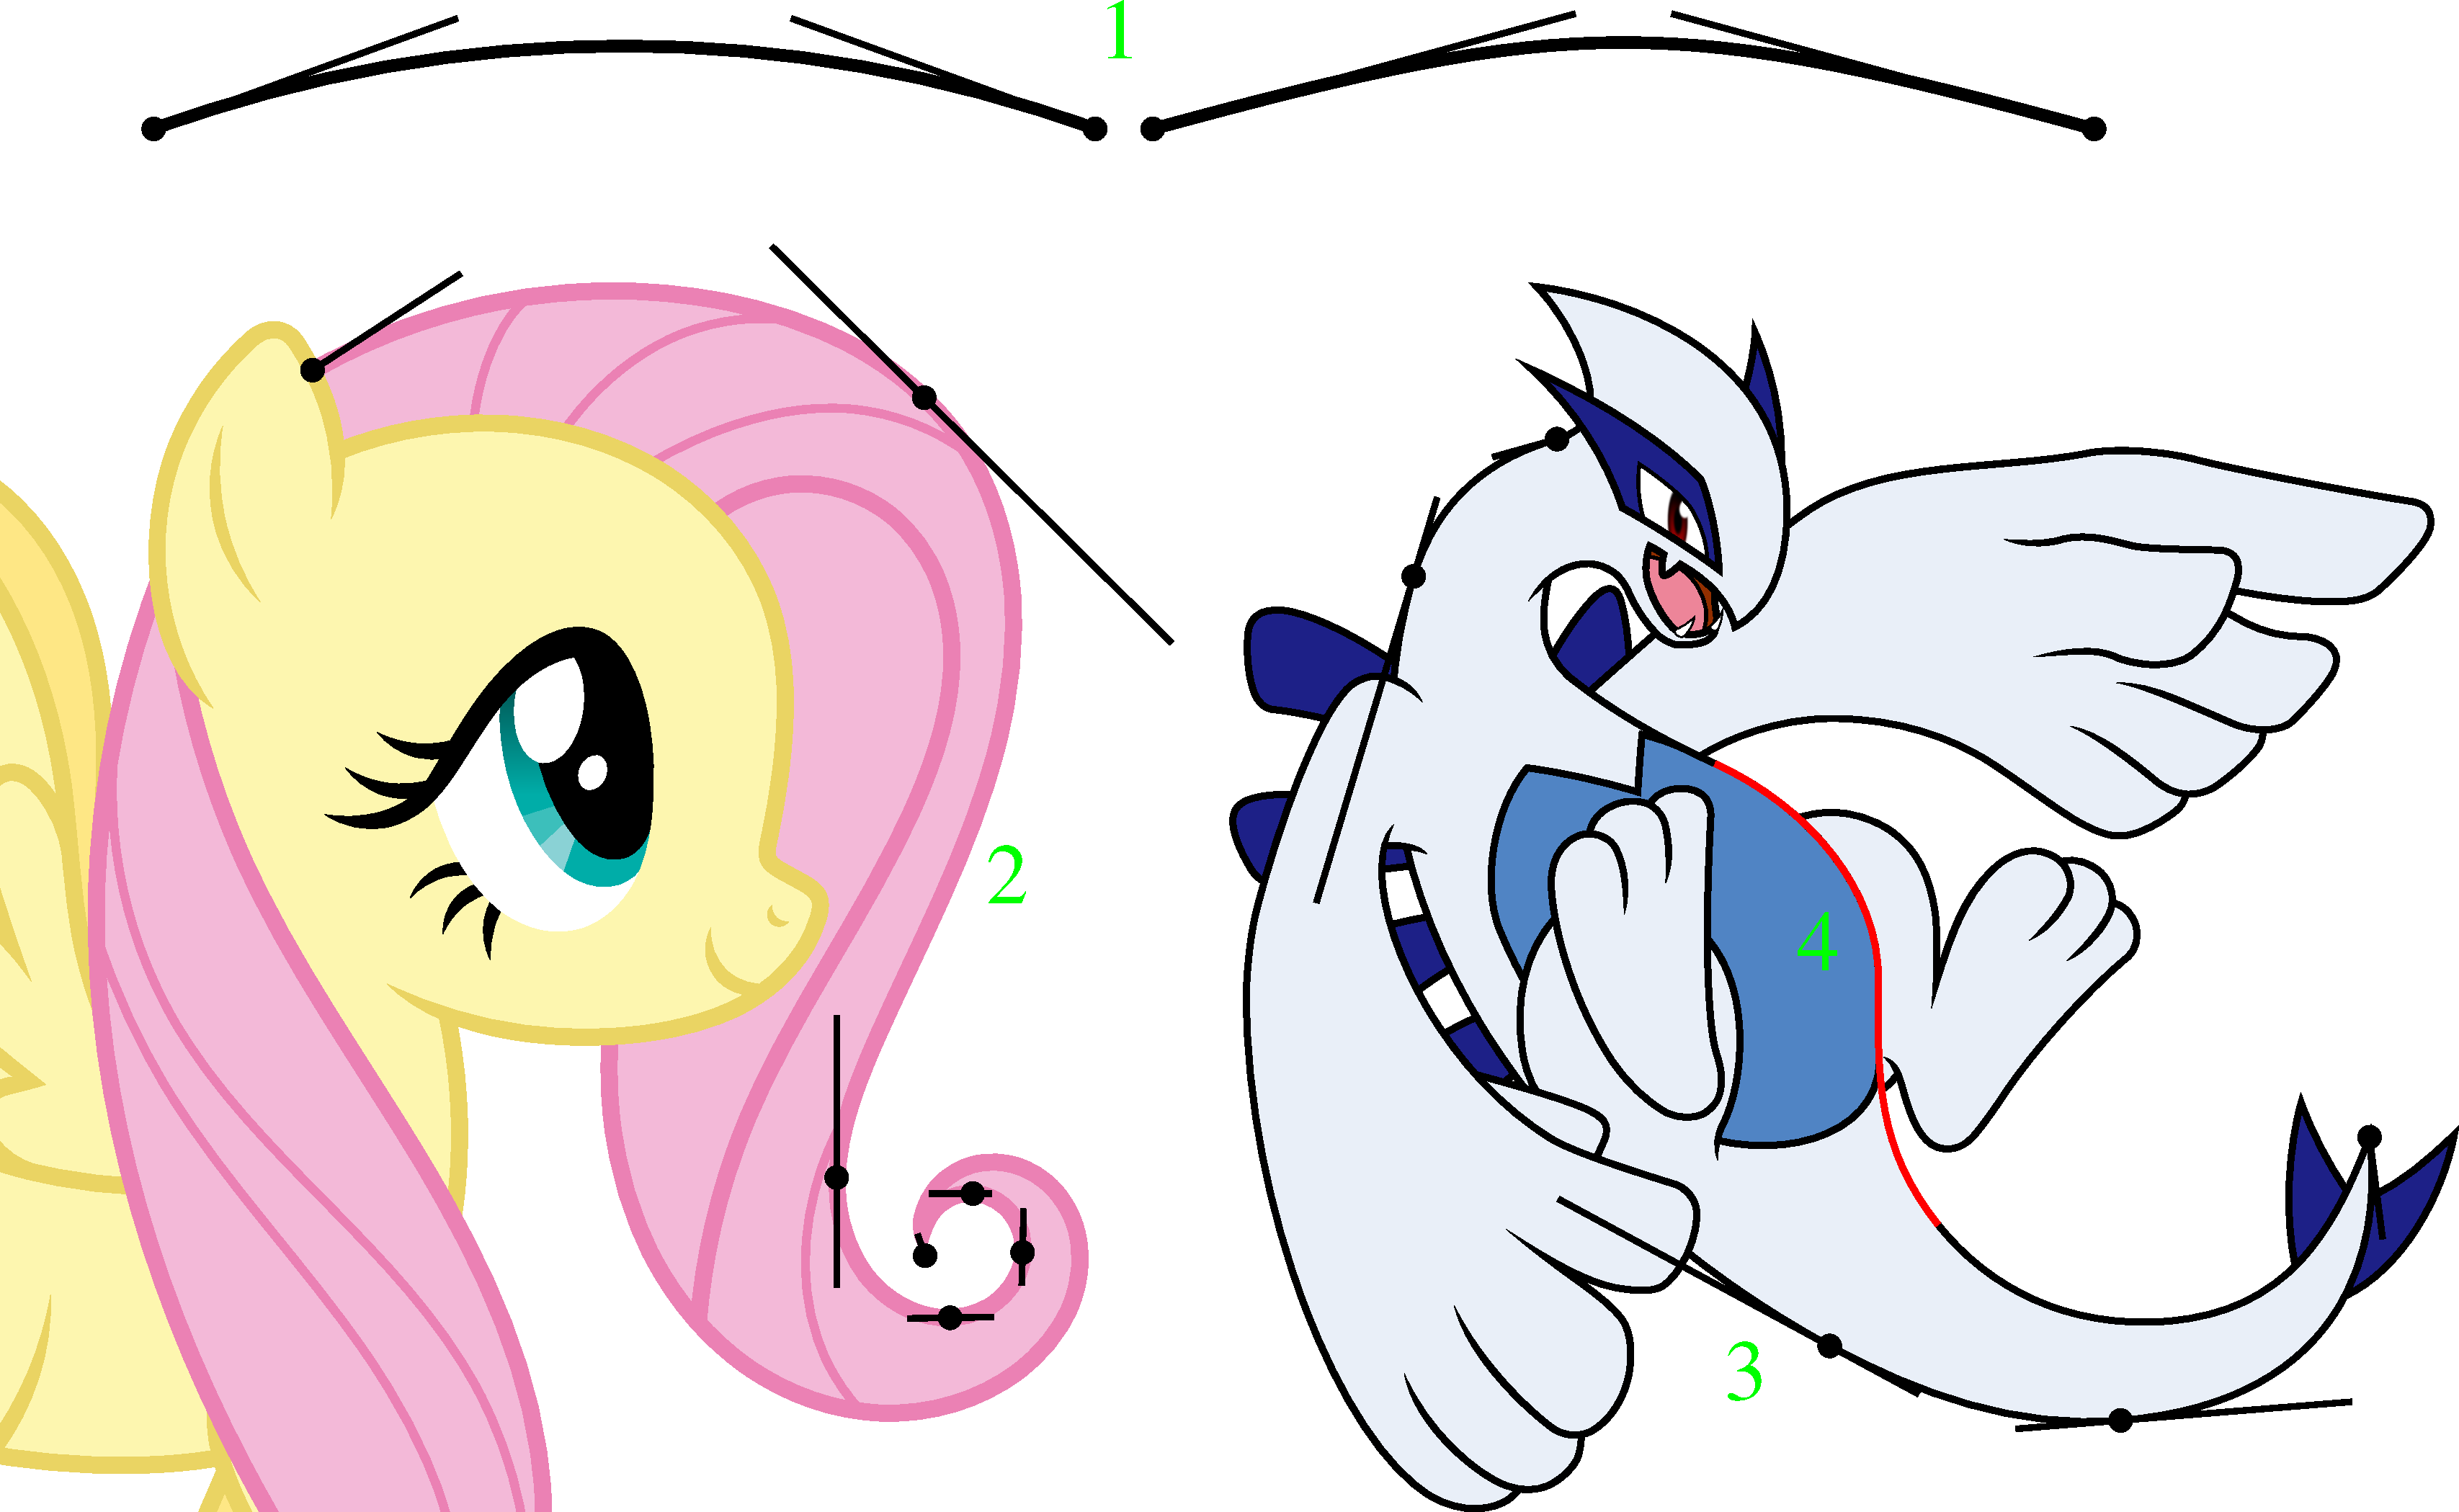
\includegraphics[width=\textwidth]{../resources/usability_bezier.pdf}
					\caption{Usability Analysis of Bézier Splines (left: Fluttershy \cite{fluttershy}, right: Lugia \cite{lugia})}
					\label{figure:usability_bézier}
				\end{figure}

				Figure \ref{figure:usability_bézier} illustrates some of these issues by showing some examples of Bézier splines as they appear in common design tools. Bézier nodes are displayed as red dots, while Bézier handles are displayed as green lines.

				Example 1 shows two Bézier splines. The left curve is a Bézier spline approximation of a circular arc, exhibiting nearly constant curvature, while the right one is not, going from low curvature to high curvature and back to low curvature. Since the difference can be hard to see, it's easy to make mistakes when trying to approximate circular arcs using Bézier splines.

				Examples 2 and 3 show curves that could be described more efficiently in terms of curvature. Since there is no way to directly specify curvature using Bézier splines, a considerable number of nodes is needed to get close to the desired curve.

				Example 4 shows a spline with a curvature discontinuity which went unnoticed by the artist at the time of creation. In fact, this discontinuity would be even less visible if the curve was not vertical at said point, manifesting itself only in a reduced overall smoothness of the curve, without a clear indication of where the problem lies.

			\subsubsection{Spiro Splines}
			\label{section:spiro_splines}

				Spiro splines were added to Inkscape in 2009. Even though they were integrated using path effects and thus have a somewhat cumbersome user interface, they constitute a commendable effort of incorporating results from curve research into vector graphics software, something that has hardly happened this far. More information on Spiro splines can be found in the dissertation of Raphael Levien \cite{thesis-spiro}.

				Spiro splines consist of parts of the Euler spiral, which is a curve whose curvature changes linearly with the curve's arc length. The user can specify control points through which the software puts an interpolating spline. There is no way to directly specify tangent angle and/or curvature. The splines are guaranteed to have curvature continuity.

				Again, the model from section \ref{section:curve_design_process} is applied. With Spiro splines, the modelling is fairly straightforward. The user supplies a set of points for which the software computes an interpolating spline. The fairness measure chooses the segments of this spline to be parts of the Euler spiral and makes sure that there is curvature continuity and no excessive winding.

				We analyze Spiro splines in terms of the criteria presented in section \ref{section:usability_criteria_curve_design_tools}. The specification language of Spiro splines being simply points on the curve, plus the fact that on sufficiently smooth curves, not very many of them are needed, the language is well-suited to be read and spoken by humans (criteria 2 and 3). The fairness measure leads to beautifully smooth curves that are ususally sufficiently close to what a human would expect given the control points (criteria 4 and 5). The software is also good and sufficiently quick at constructing these curves (there are some cases where the algorithm fails to find a meaningful curve, but these cases are fairly artificial and can usually be avoided when designing actual curves) and thus fulfills criterion 6 well enough. The only real issue lies in the insufficient expressiveness of the specification language (criterion 1), discussed further in the following paragraph.

				Section \ref{section:bézier_splines} discussed how the lack of ability to specify curvature using common Bézier spline design tools adversively affects usability. Many of the same points apply to Spiro spline design tools, since they allow the user to neither specify direction nor curvature. These properties can only be expressed indirectly, by placing the control points in such a way that the algorithm will create a curve that has the desired properties, resulting in the usability issues described previously, such as requiring many control points to be specified even though the curve could be described much more concisely in terms of direction and/or curvature. This seems especially unfortunate when considering that the spline primitive of Spiro splines, the Euler spiral, would lend itsself excellently to describing circular arcs, spirals and other shapes exhibiting constant or linearly changing curvature. Sometimes, the algorithm can be coaxed into producing the desired curve by placing just a few control points very carefully, resulting in a series of Euler spiral segments that exhibit the wanted properties. Unfortunately, this is rarely practical, since it both requires a lot of time to set up and doesn't behave very well when modified. These issues are somewhat alleviated by the guaranteed curvature continuity together with the general tendency of the algorithm to produce extremely smooth curves even when many control points are involved. That way, when indirectly specifying tangent angle and/or curvature by placing many control points, it's not as easy to accidently create small bumps as with Bézier splines.

				\begin{figure}[htb]
					\centering
					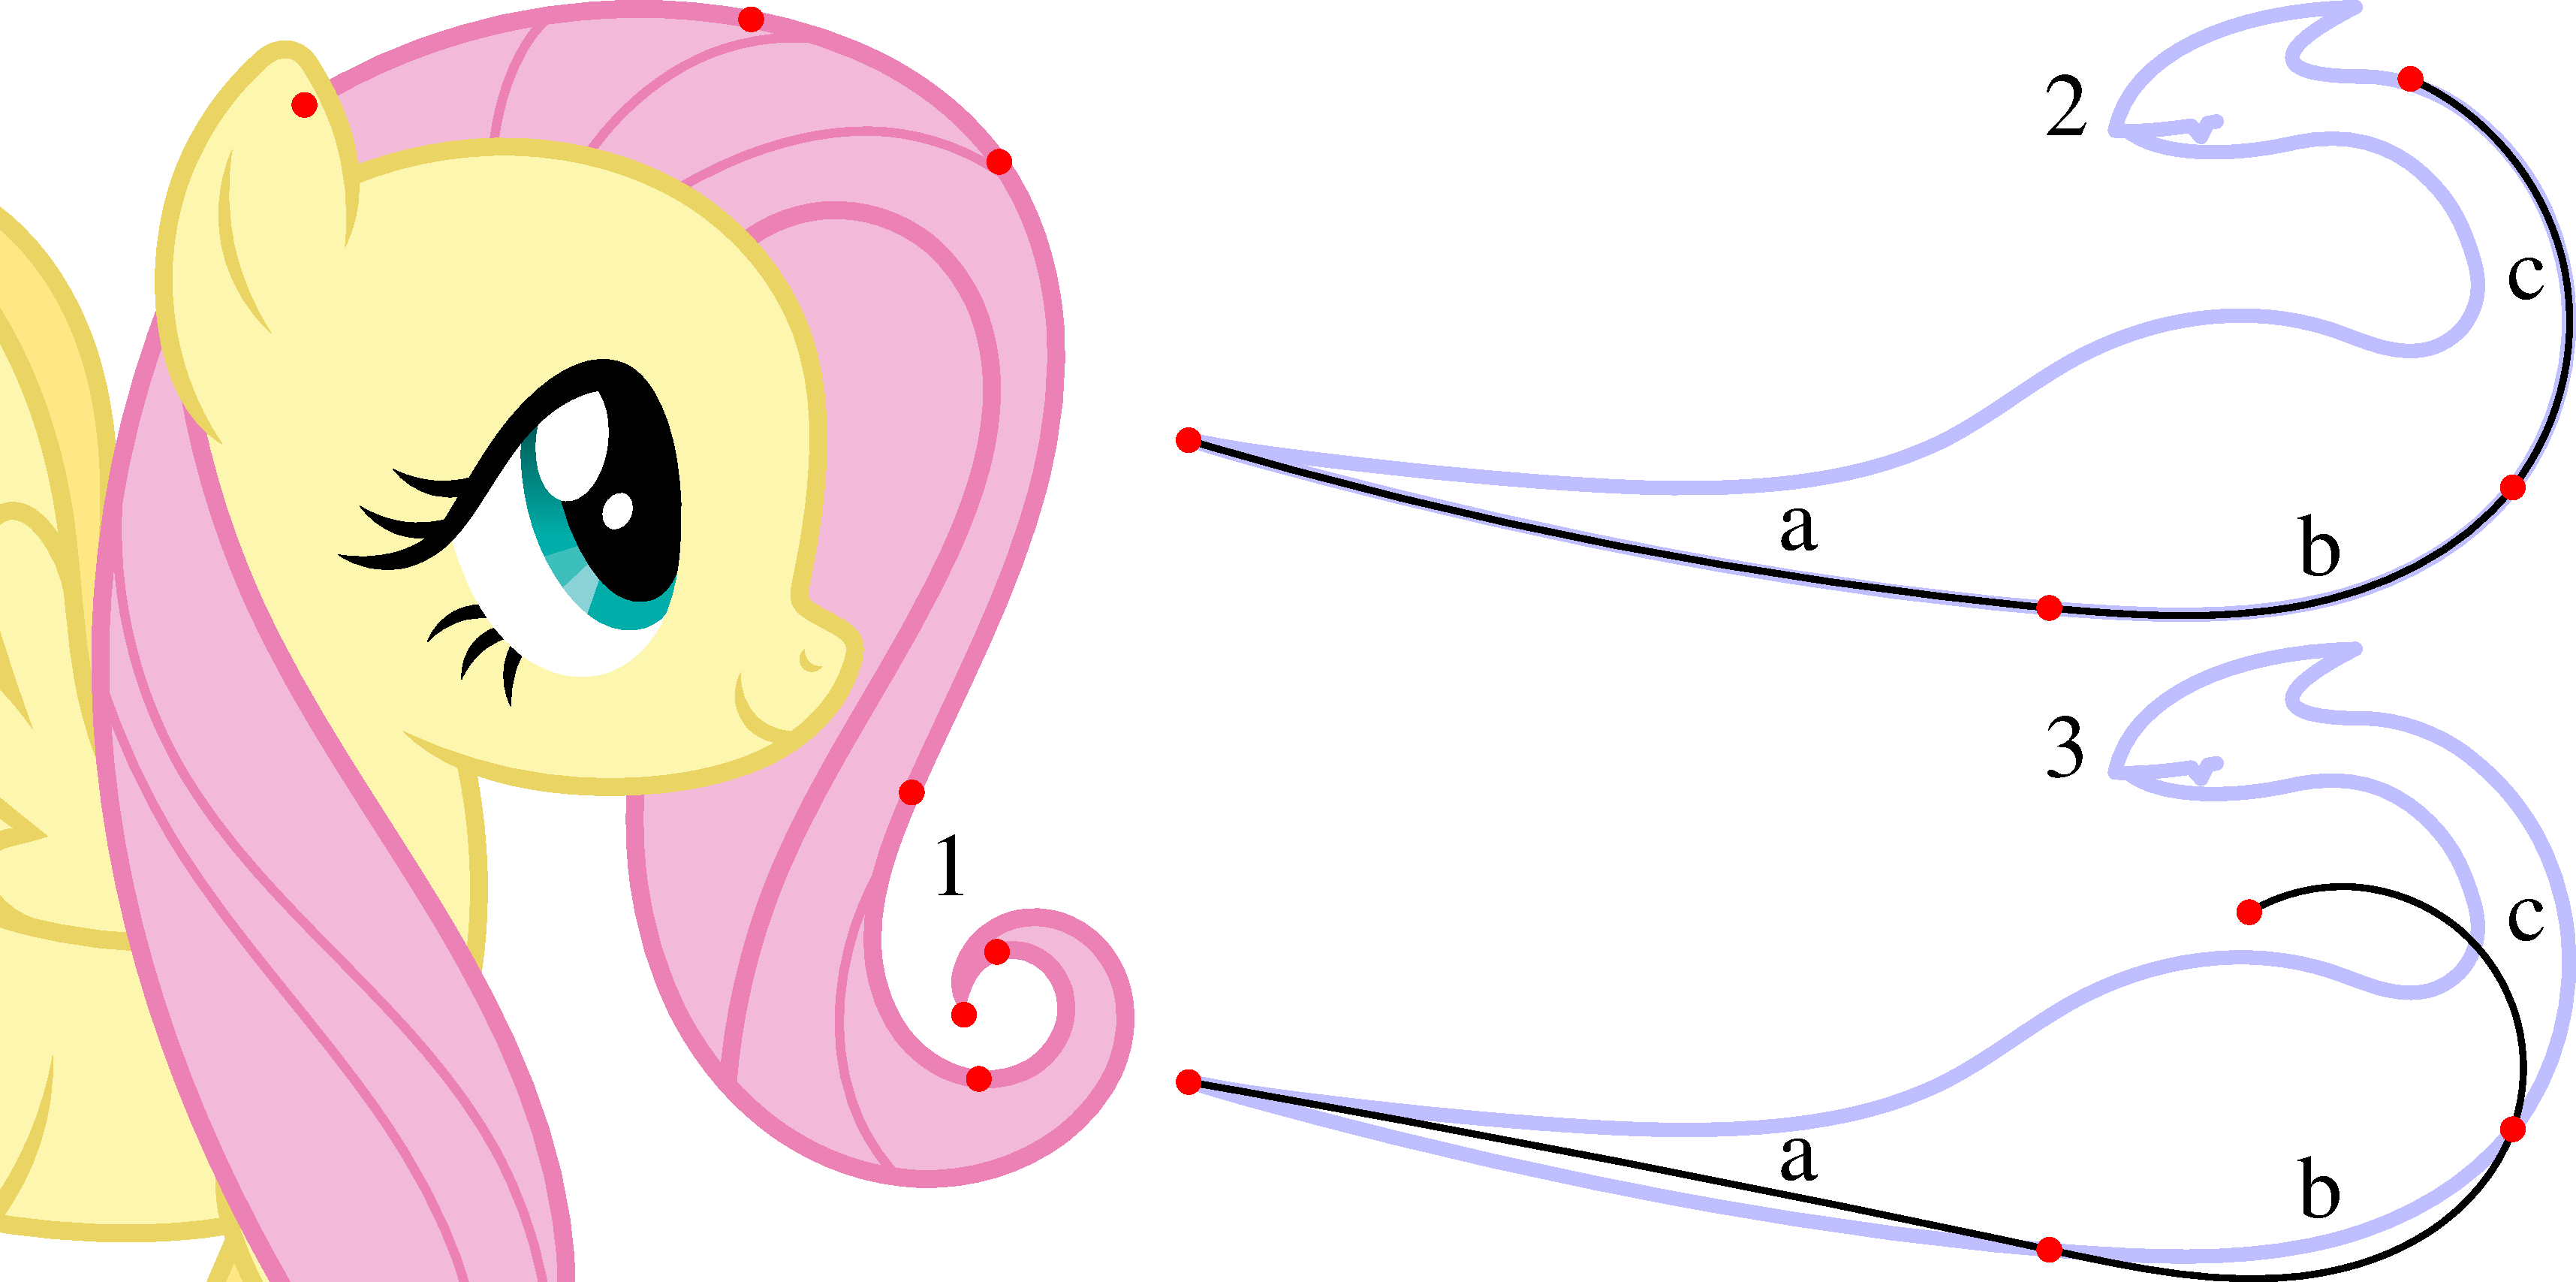
\includegraphics[width=\textwidth]{../resources/usability_spiro.pdf}
					\caption{Usability Analysis of Spiro Splines (left: Fluttershy \cite{fluttershy}, right: Lugia \cite{lugia})}
					\label{figure:usability_spiro}
				\end{figure}

				Figure \ref{figure:usability_spiro} illustrates some of these issues by showing some examples of Spiro splines as they appear in common design tools. Control points are displayed as red dots.

				Example 1 shows a shape that is in principle well-suited for being represented by parts of the Euler spiral. Unfortunately, describing the curve using Spiro splines still requires many control points. Note that even though this example has the same number of specified on-curve points (7) as the corresponding example in section \ref{section:bézier_splines}, the latter has an additional 12 velocity specifications, proving that even though curvature cannot be specified explicitly, Spiro splines are a much better choice for curves that are best expressed in terms of curvature than Bézier splines.

				Example 2 shows how some shapes can be described using Spiro splines by placing only very few control points. In this case, the shape consists of a circular arc with low curvature (segment a), a segment of linearly increasing curvature (segment b) and finally a circular arc with high curvature (segment c). This shape can be described conveniently using a Spiro spline with just 4 carefully placed control points.

				Unfortunately, as can be seen in example 3, this scenario does not handle modifications very well. For instance, increasing the curvature of segment c has to be done indirectly by moving a control point. Unfortunately, this adversely affects segment a, since the curvature there was not specified directly but instead relied on the rather fragile configuration of the 4 control points.

	\section{Proposed Solution}
	\label{section:proposed_solution}

		Having analyzed the usability aspect of curve design tools in section \ref{section:problem_analysis}, it's time to think about how to properly address their current issues. In the following sections, we propose both an abstract approach for designing usability-oriented curve design tools, as well as our specific ideas for developing a piece of software using this approach.
          
		\subsection{Description-Based Curves}
		\label{section:description-based_curves}

			Seeing how the description language almost completely determines all usability aspects of the resulting curve design tool, it seems unwise to base it on low-level mathematical aspects of the curve as is the case with Bézier splines. Spiro splines are much better in that a lot of effort was put into the fairness measure. Unfortunately, the project has set out to solve the problem of constructing interpolating splines, thereby committing to a very restricted specification language right from the start.

			We think that in order to get the best usability, using a good specification language which does not rely on implementation details has to be the top priority. Together with a good fairness measure, it forms a description language that, if it allows for reliable and efficient derivation of curves, will then lead to usable curve design tools. Since it is not immediately clear which description language is the best, the first step is to move away from the traditional explicit curve construction, and instead use a process that enables the creation of curves based on descriptions.

			\begin{figure}[htb]
				\centering
				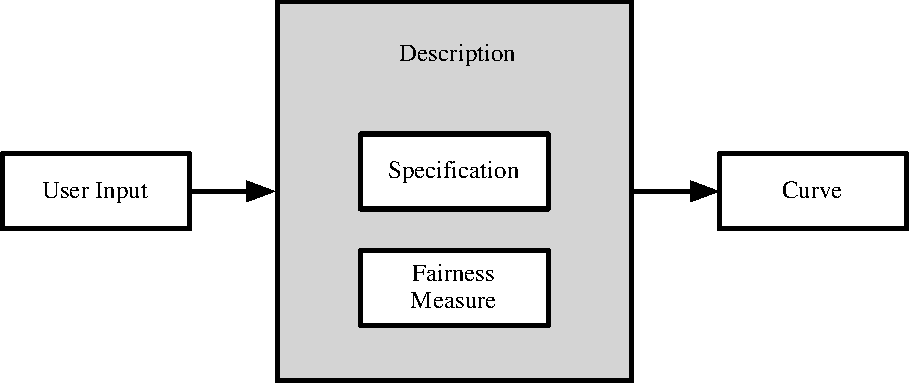
\includegraphics[width=\textwidth]{../resources/description-based_curves.pdf}
				\caption{Description-Based Curves}
				\label{figure:description-based_curves}
			\end{figure}

			Figure \ref{figure:description-based_curves} shows such a process. Note that this approach doesn't give any specifics yet, since the previous usability analysis didn't give a complete answer as to what the optimal curve design tool looks like. It has yet to be determined what the description language should be, as well as how to derive curves from these descriptions.

		\subsection{Description Language}
		\label{section:description_language}
			
			After establishing the general approach to curve design tools in section \ref{section:description-based_curves}, it's time to decide on the specifics in order to create an instance of this model. The first step is to choose a description language, consisting of both a specification language and a fairness measure.

			The human visual system seems to be fairly insensitive to properties beyond the second derivative of the curve, that is, beyond curvature. Based on that premise, we chose to let the user specify properties up to the second derivative of the curve using the specification language. The fairness measure will then select the curve whose third derivative is minimal from the set of curves that fulfill the specification's requirements.

			\subsubsection{Specification Language}
			\label{section:specification_language}

				The specification language we propose uses differential geometric properties of parametric curves and is thus decoupled from specifics of the underlying curve model, hopefully leading to a specification language that is easier to learn and use. The specification language will focus on the properties point, direction and curvature as defined in \ref{section:parametric_plane_curves}. In order to provide maximal flexibility, the specification language should allow to specify any combination of these three properties at any number of positions on the curve.

				When only concerned with point specifications, it's sometimes enough to require the curve to go through all of them in order, although sometimes, this will lead to undesirable results. Even with the curve preserving the order in which the points are visited, it is unspecified how much arc length the curve will spend between each pair of points. When specifying direction and/or curvature without an associated point, it becomes a necessity to associate this specification with some kind of positional information in order to anchor it to some point on the curve. If this was not done, the specification could move freely along the curve and would thus behave very unpredictably. We thus chose to associate each combination of point, direction and curvature with a position on the curve.

				With that in mind, it is now possible to abandon this notion of a combination of point, direction and curvature and instead talk about specification items, a specification item being either a positioned point, a positioned direction or a positioned curvature. For example, a combination of point and curvature at some position thus splits up into a point specification item at this position and a curvature specification item at the same position.

				An obvious choice for specifying a position on a curve would be by giving a parameter value for the underlying parametric curve. However, this would violate our design idea of using differential geometric properties of curves. A way of specifying a position on a curve that is independent from its parametrization is the arc length of the curve. Instead of directly using the arc length to give the positions of specification items, we chose to specify positions as fractions of the total arc length of the curve. This way, the position of a specification item relative to the start and end points of the curve is independent of the total arc length of the curve.

				% TODO: explain this in more detail (o--o----------------o, pull last specification, makes wobbly segment at beginning) 
				With this setup, it seems advisable to also include the curve's total arc length in the specification. This way, one can specify curves that don't have any specification items associated to their start and end points. Also, with unspecified curve length, changing any specification item may inadvertently change the curve's total arc length, thus possibly adversely affecting other parts of the curve whose specification item positions are given as a fraction of the curve's total arc length.

				Thus, the final specification language is as follows:
				\begin{equation*}
					\begin{alignedat}{2}
						& \mathrm{Positions}          && = \unit\\
						& \mathrm{Points}             && = \R{2}\\
						& \mathrm{Directions}         && = \RR\\
						& \mathrm{Curvatures}         && = \RR\\
						& \mathrm{SpecificationItems} && = \mathrm{Positions} \times \left(\mathrm{Points} \cup \mathrm{Directions} \cup \mathrm{Curvatures}\right)\\
						& \mathrm{CurveLengths}       && = \RR\\
						& \mathrm{Specifications}     && = \powerset{\mathrm{SpecificationItems}} \times \mathrm{CurveLengths}
					\end{alignedat}
				\end{equation*}

			\subsubsection{Fairness Measure}
			\label{section:fairness_measure}

				Different fairness measures for plane curves have been proposed throughout history. Many of them set out to emulate the behavior of mechanical splines made from wood or steel, which were used for industrial design before the advent of computer aided design. The most direct approach of this type uses mechanics to derive a term for the energy in an idealized bent steel band to minimize, arriving at the following functional describing the minimum energy curve (MEC) \cite{paper-mec}:
				\begin{equation*}
					\integral{0}{1}{\apply{\chi}{t}^2}{t}
				\end{equation*}
				While this approach is a good idealization of the mechanical spline, it has some disadvantages when used for curve design. For instance, it will not yield a circular arc when the curve is constrained by co-circular points. Generally speaking, the MEC fairness measure is not very sensitive to bumps and inflection points on the curve, as long as they're small. The human visual system on the other hand, very much is and would always prefer one large circular arc over five small bumps on the curve.

				In order to adress these issues, there has also been some research into fairness measures whose design is more directly motivated by the human perception of smoothness in plane curves. One such approach is that of the minimum variation curve (MVC) \cite{thesis-mvc}, whose functional is given below:
				\begin{equation*}
					\integral{0}{1}{\apply{\chi'}{t}^2}{t}
				\end{equation*}
				Minimum variation curves capture the intuitive notion of smoothness very well. The functional will put straight lines through points that are co-linear and circular arcs through points that are co-circular when otherwise unconstrained. When constraints cause different points on the curve to have different curvatures, the functional will prefer linearly changing curvature, since that will make the derivative of the curvature a constant and thereby minimize the integral over its square. In general, the MVC fairness measure is very good at avoiding bumps and inflection points when possible. Because of these appealing properties, the MVC fairness measure was chosen as part of our description language.

		\subsection{Curve Derivation}
		\label{section:curve_derivation}

			Implementing the approach presented in section \ref{section:description-based_curves} requires a way of turning descriptions into actual curves. We chose to use nonlinear optimization on polynomial splines in order to achieve this goal.

			Nonlinear optimization allowed us to stay relatively flexible with respect to the description language and enabled us to experiment with different specification languages and fairness measures, assessing their usability before settling on the choices presented in section \ref{section:description_language}.

			% TODO: make it clear that splines imply segmentation
			Polynomial curves were chosen since they are mathematically simple, very flexible through the choice of their degree, and well-suited to approximate a variety of smooth curves. We opted to use polynomial splines since they allow approximating more complex curves without involving polynomials of excessively high degree, which are known to have poor stability.

			\subsubsection{Optimization Problem}
			\label{section:optimization_problem}

				Nonlinear optimization problems are usually expressed using an objective function \(f : \function{\R{n}}{\RR}\), a constraint function \(g : \function{\R{n}}{\R{m}}\) and constraint bounds \(g_l, g_u \in \R{m}\). The optimization problem is then given by the task of finding an \(x^* \in \R{n}\) such that:
				\begin{equation*}
					\begin{gathered}
						x^* = \argmin_{x \in \R{n}} \apply{f}{x}\\
						g_l \leq \apply{g}{x^*} \leq g_u
					\end{gathered}
				\end{equation*}
				This allows for the expression of a variety of optimization goals. The ones that are important for us are zero-error constraints (using the constraint function and bounds to specify that an error term should be zero), upper bounds on errors (using the constraint function and bounds to specify an upper bound for an error term) and minimization goals (using the objective function to express that an error term should be minimized).

				Our implementation of choice uses smooth optimization, or, more specifically, an interior point method. This type of algorithm further requires the functions \(f\) and \(g\) to be at least once, ideally twice continuously differentiable.

				In the following, we will describe how nonlinear optimization can be used for finding polynomial splines based on descriptions in the language established in section \ref{section:description_language}.

			% TODO: consider structuring and naming this section similarly to the slides
			\subsubsection{Segmentation and Notation}
			\label{section:segmentation_notation}

				%\begin{equation*}
				%	\apply{\phi_i}{t} = \sum_j a_{i,j} \cdot t^j
				%\end{equation*}

				Since the polynomial spline is uniquely determined by the coefficients of each polynomial segment, the optimization domain is a vector consisting of all these coefficients. Let \(m\) be the number of segments that make up the polynomial spline. We will use the functions defined in section \ref{section:parametric_plane_curves} with subscript \(i\) when referring to the \(i\)th segment (\(\apply{\phi_i}{t}\)) and without subscript when referring to the whole spline (\(\apply{\phi}{t}\)). Mapping the parameter \(t\) between the segments and the whole spline works as follows:
				\begin{equation*}
					\apply{\phi}{\frac{i + t}{m}} = \apply{\phi_i}{t}
				\end{equation*}
				That is, the segments are simply laid out consecutively in parameter space, scaled to fit the unit interval, making the parameter mapping function linear and static.

				Let \(n\) be the number of specification items. Let \(\hat{t}_i\) be the position of the \(i\)th specification item. If the \(i\)th item is a point specification, the point is denoted \(\hat{\phi}_i\), if it is a direction specification, the direction is denoted \(\hat{\delta}_i\) and if it is a curvature specification, the curvature is doneted \(\hat{\chi}_i\). The specified total arc length for the curve is denoted \(\hat{\lambda}\).

			\subsubsection{Constant Speed}
			\label{section:constant_speed}

				Since we chose to give the position of a specification item as a fraction of the curve's total arc length, we need the function mapping the covered arc length to the corresponding parameter values in order to state the optimization goals for the specification items. Unfortunately, this function is not very well-suited to be used as a term in a smooth opimization problem even for simple curves like polynomials. Also, since the function isn't fixed and varies with the coefficients, there is no way of telling on which segment each specification item will end up, something that is also difficult to state in a smooth optimization problem. We also need to state the specification of the total arc length of the curve as an optimization goal, which may be difficult if the the covered arc length function is hard to express. Furthermore, the difficulty of expressing the fairness measure, which is often an integral over the arc length of the curve, is dependent on the complexity of the covered arc length function. In order to address all these problems, the following error term is used:
				\begin{equation*}
					\max_{t \in \unit} \xa{\apply{\sigma}{t} - \hat{\lambda}}
				\end{equation*}
				For polynomial splines with sufficient degree and segment count, this term will be brought close to zero in the optimization, making the speed approximately constant with value \(\hat{\lambda}\). This, in turn, makes the covered arc length function approximately linear (\(\apply{\lambda}{t} \approx \hat{\lambda}t\)), facilitating the simple statement of the optimization goals for the specification items and the fairness measure as well as fixing the segment for each specification item. It also causes the total arc length of the curve to be approximately equal to \(\hat{\lambda}\), as requested by the specification.

				Since this goal can only be fulfilled approximately by polynomial curves, it is impossible to use the error term given above in a zero-error constraint. It could however be used in both an upper bound on errors and in a minimization goal. Both approaches were implemented and tested, with the latter yielding a more stable optimization process.

				The error term given above is not well-suited for smooth optimization because it incorporates finding a maximum. Since the optimization problem will allow the original error term to be brought close to zero, we can approximate it using the following error term:
				\begin{equation*}
					\hat{\lambda}^{-2}\integral{0}{1}{\xp{\apply{\sigma}{t} - \hat{\lambda}}^2}{t}
				\end{equation*}
				Since this term is intended to be used as a minimization goal, the factor \(\hat{\lambda}^{-2}\) was added, which makes it scale invariant. This enables the error term to be statically weighted against other terms in the objective function without this weighting being shifted because of curve scaling.

			\subsubsection{Continuity Connections}
			\label{section:continuity_connections}

				As mentioned in section \ref{section:description_language}, we are not concerned with properties beyond the second derivative of the curve. Thus, we will only require \(\contg{2}\) continuity for the whole spline. While the polynomial curves used as segments are smooth (\(\contp{\infty}\) continuity), the resulting spline in general is not. The segments have to be pieced together in such a way as to ensure a certain degree of smoothness. Thus, to ensure \(\contg{2}\) continuity for the whole curve, it is sufficient to ensure \(\contg{2}\) continuity at the segment connection points. To do this, the following error terms are added for each connection point (\(0 \leq i \leq m - 1\)):
				\begin{equation*}
					\begin{gathered}
						\apply{\phi_i}{1} - \apply{\phi_{i + 1}}{0}\\
						\apply{\phi'_i}{1} - \apply{\phi'_{i + 1}}{0}\\
						\apply{\phi''_i}{1} - \apply{\phi''_{i + 1}}{0}
					\end{gathered}
				\end{equation*}
				These error terms being zero implies \(\contp{2}\) continuity. However, since the constant speed requirement introduced in the previous paragraph collapses \(\contp{2}\) continuity and \(\contg{2}\) continuity, this is equivalent to the original requirement of ensuring only \(\contg{2}\) continuity, yet better suited for optimization. 

				Since it is not acceptable for the curve segments to not touch, have sharp corners or curvature discontinuities, the error terms above are added as zero-error constraints.

			\subsubsection{Specification Items}
			\label{section:specification_items}

				Having taken care of the somewhat technical details arising from using polynomial splines, it's time to state the error terms for the specification items. Since the optimization goal in section \ref{section:constant_speed} makes sure that \(\apply{\lambda}{t} \approx \hat{\lambda}t\), we know that the whole spline is parametrized in such a way that the parameter \(t\) is a fraction of the curve's total arc length. This fits perfectly with the fact that the position of each specification item is also specified as a fraction of the curve's total arc length. Thus, for each specification item (\(0 \leq i \leq n\)), we add one of the following error terms, depending on the type of the specification item:
				\begin{equation*}
					\begin{gathered}
						\apply{\phi}{\hat{t}_i} - \hat{\phi}_i\\
						\apply{\delta}{\hat{t}_i} - \hat{\delta}_i\\
						\apply{\chi}{\hat{t}_i} - \hat{\chi}_i
					\end{gathered}
				\end{equation*}

				The user usually wants to specify exact curve behavior rather than indirectly influencing properties, so these error terms are also added as zero-error constraints.

			\subsubsection{Fairness Error}
			\label{section:fairness_error}

				Since constant speed was established in section \ref{section:constant_speed}, stating the error term for the fairness chosen in section \ref{section:fairness_measure} is fairly straightforward:
				\begin{equation*}
					\hat{\lambda}^2\integral{0}{1}{\apply{\chi'}{t}^2}{t}
				\end{equation*}
				It's clear that in many cases, this error term will not be zero, and in fact, may be arbitrarily large. Thus, it is not suitable to be constrained to zero or bounded error and has to be stated as a minimization goal. Note that similar to the error term for constant speed, we added the factor \(\hat{\lambda}^2\), which causes the fairness measure to be invariant under scaling of the whole curve, enabling static weighting of error terms in the objective function.

			\subsubsection{Final Assembly}
			\label{section:final_assembly}

				Having gathered all the necessary error terms, it's time to put them together. Terms with zero-error constraints, as well as terms with upper bounds on the error are added as component functions of the constraint function \(g\) together with appropriate bound components in \(g_l\) and \(g_u\).

				Minimization goals, on the other hand, are assembled in a weighted sum which defines the the objective function \(f\). Since the error terms were designed to be scale invariant, this weighting can be done statically. The exact values of the weights are to be determined empirically.

	\section{Implementation}

		\subsection{Architecture}
			
			\subsubsection{Programming Language}
			
				The first step of the implementation of the proposed solution is the choice of the platform and development environment that will be used. 
				As the programming language, C\# is the best option due to the following features:
				
				\begin{itemize}
				  	\item Platform independence - the project is not bound to any specific platform and can be used on all major operating systems, provided the libraries Kurve depends on are available. 
				  	\item C\# is a high-level language - this reduces overhead in the development process, for example spending time on manual memory management.
					\item Ability to interface with native code - native code can be interfaced with by using reasonable amounts of boilerplate code. As it was clear that native libraries would be used, this is a key requirement.
					\item Familiarity - the developers are familiar with this language. This choice eliminates overhead that would be caused by adopting an unfamiliar language.
					\item UI frameworks - part of the project is a proof of concept user interface to work with curves. Several UI frameworks are available that interface directly with C\#.
				\end{itemize}
			
			\subsubsection{Libraries}
				
				Kurve offers its own APIs in C\# for working with terms and optimization problems. However, the implementations of the functionalities of these APIs are provided by third-party libraries. Hence, Kurve relies on several libraries, including:
				
				\begin{itemize}
				  	\item Ipopt\footnote{https://projects.coin-or.org/Ipopt} is a library that does numeric non-linear optimization. This library finds optima of optimization problems based on an objective function and its first two derivatives. In addition, it allows the specification of hard constraint functions (and their first two derivatives) that the solutions have to match. This allows Kurve to use hard specifications on curves.
					\item CasADi\footnote{http://casadi.org} provides functionality to perform automatic differentiation of terms. It interfaces with Ipopt directly, which makes it a perfect match for Kurve's symbolic differentiation needs. CasADi is written in C++, but unfortunately only C functions can be called easily from C\#. For that reason, a small CasADi wrapper written in C was required to implement Kurve's C\# term APIs. 
				\end{itemize}
			
				 Kurve has strong requirements for both libraries: Terms used in the functions that need to be optimized in Kurve are quite large and plentiful, but differentiation and optimization still need to be performed in a short period of time to allow real-time editing of curves. Fortunately, CasADi and Ipopt are very efficient and allow Kurve to offer close to real time editing of curves.

				For Kurve's user interface, GTK\#\footnote{http://www.mono-project.com/GtkSharp} was used. GTK\# is used to draw the curves and controls into a window, as well as handling keyboard and mouse events.
				
			\subsubsection{Subsystem Decomposition}	
			
				\begin{figure}[htb]
					\centering
					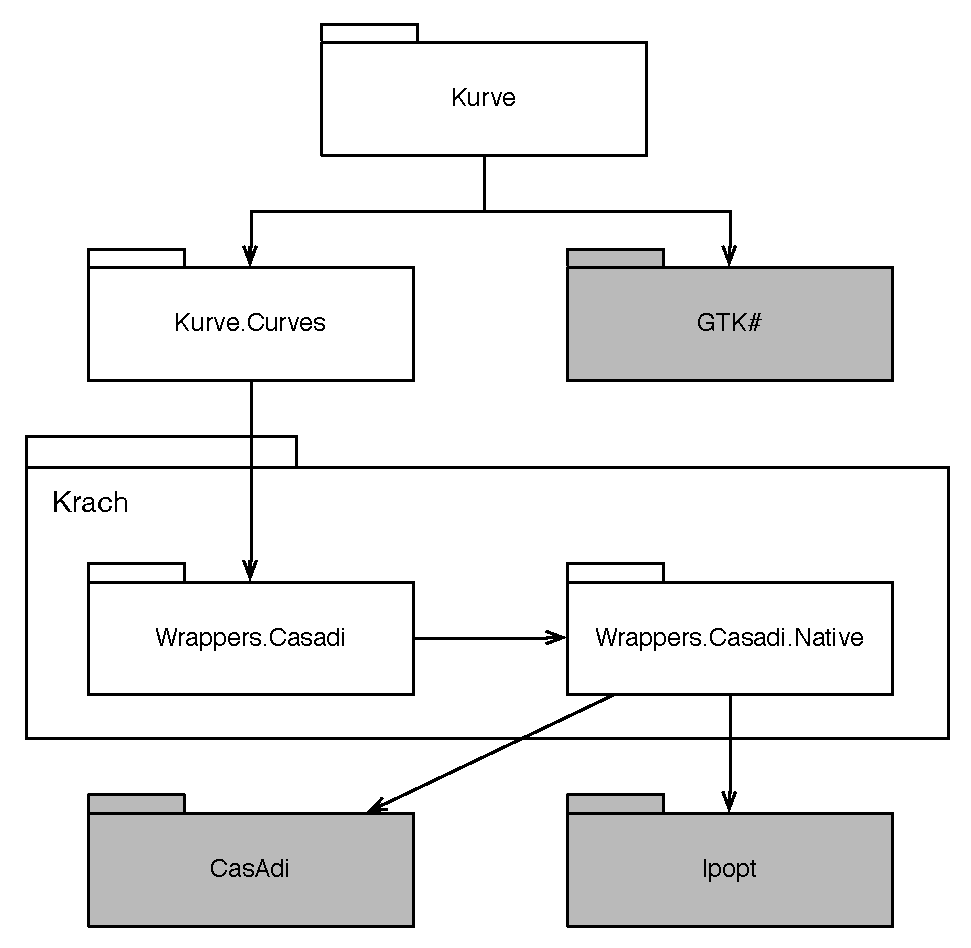
\includegraphics[width=\textwidth]{../resources/subsystems.pdf}
					\caption{Subsystem Decomposition of the Kurve Project}
					\label{figure:subsystem_decomposition}
				\end{figure}
				
				Kurve's implementation is split into two primary subsystems: Kurve contains the user interface related code and has a dependency on GTK\# as well as Kurve.Curves; Kurve.Curves is responsible for generating curves from specifications using CasADi through Wrappers.Casadi. 
				
				Wrappers.Casadi and Wrappers.Casadi.Native contain a wrapper for CasADi using C\# and C++ code respectively. Wrappers.Casadi uses the functions defined in Wrappers.Casadi.Native. Wrappers.Casadi and Wrappers.Casadi.Native are now part of the general-purpose library Krach to allow easy reuse in other projects.
		
		\section{Numerical Optimization}
			The Curve.Curves project contains the code required to transform input specifications into curves. It relies on CasADi (through Krach.Wrappers.Casadi) to represent curves symbolically and on Ipopt for optimization.
			
			\subsection{Specification}
				\begin{figure}[htb]
					\centering
					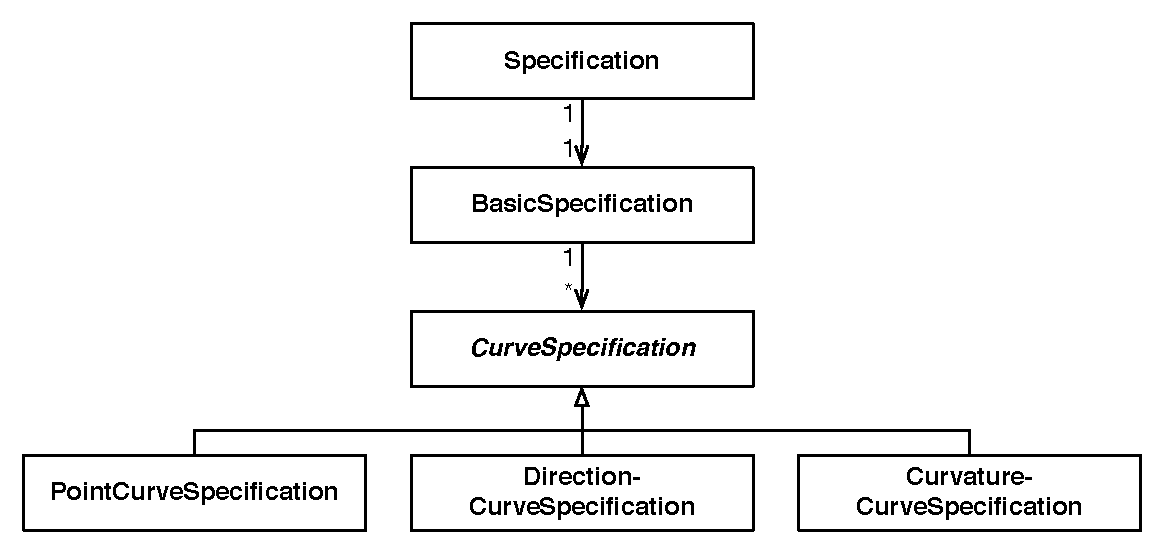
\includegraphics[width=\textwidth]{../resources/specification_class_diagram.pdf}
					\caption{Class Diagram of Specification-Related Classes}
					\label{figure:specification_class_diagram}
				\end{figure}
				
				To fully specify a curve, several different pieces of information are needed:
				
				\begin{itemize}
					\item Any number of point, direction and curvature specifications. A set of such CurveSpecifications is stored in a BasicSpecification.
					\item The curve's total length is also part of a BasicSpecification.
					\item The curves are represented using a number of segments, each of which is represented by some function, realized using the FunctionTermCurve class. Because of that, the number of segments as well as the function type that is used to represent each segment are part of the BasicSpecification as well. 
					The type of function used is represented using a FunctionTermCurveTemplate object; this template allows the creation of FunctionTermCurve objects.  
					However, this information is only used during optimization; if the number of segments and function template yield a curve with enough degrees of freedom with respect to the other specifications, roughly the same curve will be generated even if the number of segments and function template is changed. It is possible to specify the segment count and function template to modify the degrees of freedom that the resulting curves offers (i.e. more degrees of freedom mean the curve can satisfy more curve specifications while maintaining constant speed and good fairness, but the optimization process takes longer).
					\item Curves could be generated from a BasicSpecification alone. However, if there are multiple curves that fit a BasicSpecification very well (i.e. the optimization problem has multiple local optima), different actual curves could be generated from a BasicSpecification. This results in a number of problems: for example, when saving a curve, if only the BasicSpecification were saved, it would be possible that a different curve is displayed when loading the curve, because a different local optimum was reached in the optimization process. This is clearly undesirable and a way to disambiguate between the different optima is required. 
					For that reason, a full Specification consists of a BasicSpecification as well as some disambiguation information. That disambiguation information is the result of the optimization, which can be used as a starting position for the optimization process when a curve is loaded. This both ensures that the same curve will be generated and speeds up the optimization process as well.
				\end{itemize}
				
				
			\subsection{Optimization}
				\begin{figure}[htb]
					\centering
					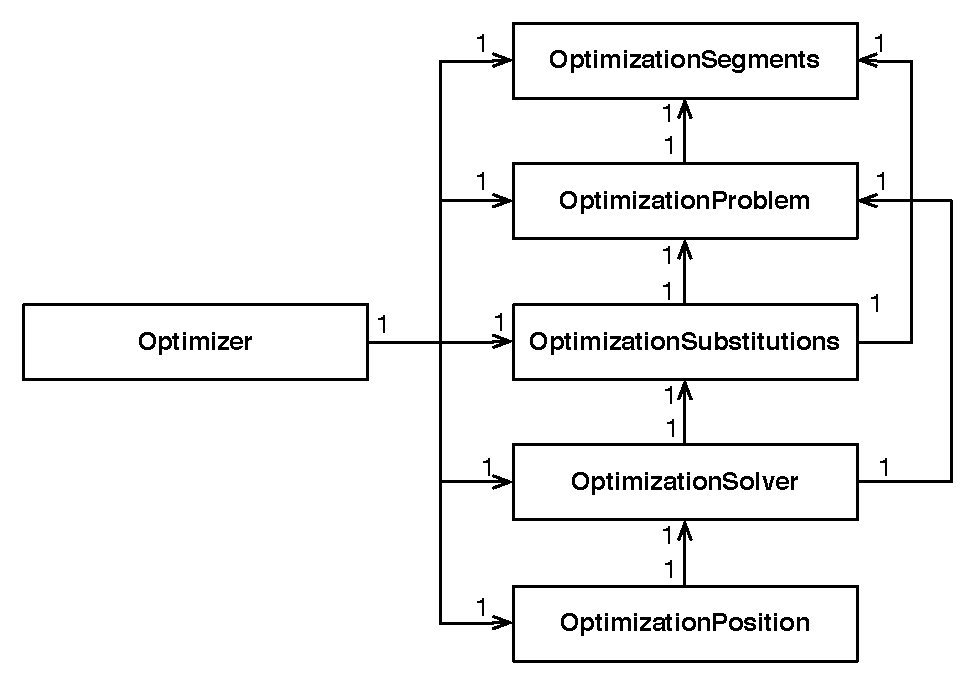
\includegraphics[width=\textwidth]{../resources/optimization_class_diagram.pdf}
					\caption{Class Diagram of Optimization-Related Classes}
					\label{figure:optimization_class_diagram}
				\end{figure}
				
				The Optimizer class handles the optimization process of a curve. By supplying a Specification, a concrete curve as well as a new Specification with updated disambiguation information can be obtained. The resulting curve is represented by a Curve object which allows access to the curve's points, speed, direction and curvature, but carries no information about the internal segmentation and function type used.
				
				The optimization process is perfomed in a number of steps. Depending on the change of the specification, only certain steps have to be run again as previous results can be reused.
				
				
				\subsubsection{Segments}
					The first step, OptimizationSegments, creates curve segments based on the number of segments and the segment template specified in the BasicSpecification. A list of parameters of all segments is created; by applying concrete values to each of the parameters, a concrete curve can be obtained. The generated segments are cached and do not have to be regenerated if the number of segments and segment template specified in the basic specification do not change.
					
				\subsubsection{Optimization Problem}
					Next, the optimization problem is created. The optimization problem specifies an objective function which includes the speed error discussed in section \ref{section:constant_speed} as well as the fairness function discussed in section \ref{section:fairness_measure}. Furthermore the continuity connections discussed in section \ref{section:continuity_connections} and the satisfaction of the specifications of the curve are realized using a constraint function. This step also computes the first and second derivatives of those functions. The concrete values required by the curve specifications are not used; instead, placeholder variables are introduced. For the total length of the curve a placeholder is used as well. This allows the reuse of the optimization problem if curve specifications or curve length change; the derivatives do not have to be recomputed. Thus, the optimization problem is cached and only rebuilt if the optimiztion segments change or if the number of each type of constraint on the curve changes. If the value of a constraint changes, but the type of constraint remains the same (e.g. a point constraint requires the curve to pass through a different point than before), the optimization problem does not have to be rebuilt.
					
				\subsubsection{Substitutions}
					In this step, substitutions for each of the placeholder variables (i.e. for each curve specification and the curve length) are created. These substitutions, when applied to an optimization problem, remove all placeholder variables and yield the optimization problem that needs to be solved to obtain a concrete curve. The substitutions have to be rebuilt whenever a specification changes, the total curve length changes, or any of the previous steps had to be recomputed.
					
				\subsubsection{Solver}
					In this step, a solver for the optimization problem is created. The solver used is provided by Ipopt. A new solver needs to be created whenever either the optimization problem or the substitutions change.
				
				\subsubsection{Position}
					The position represents a result of an optimization process. To obtain this, the solver created in the previous step is run; as the starting position, the previous optimization's position is used. Using the obtained position, a concrete curve can be obtained from the optimization segments. This curve is the desired end result returned by the Optimizer. 
				
		\section{User Interface}
			\subsection{Implementation}
				\begin{figure}[htb]
					\centering
					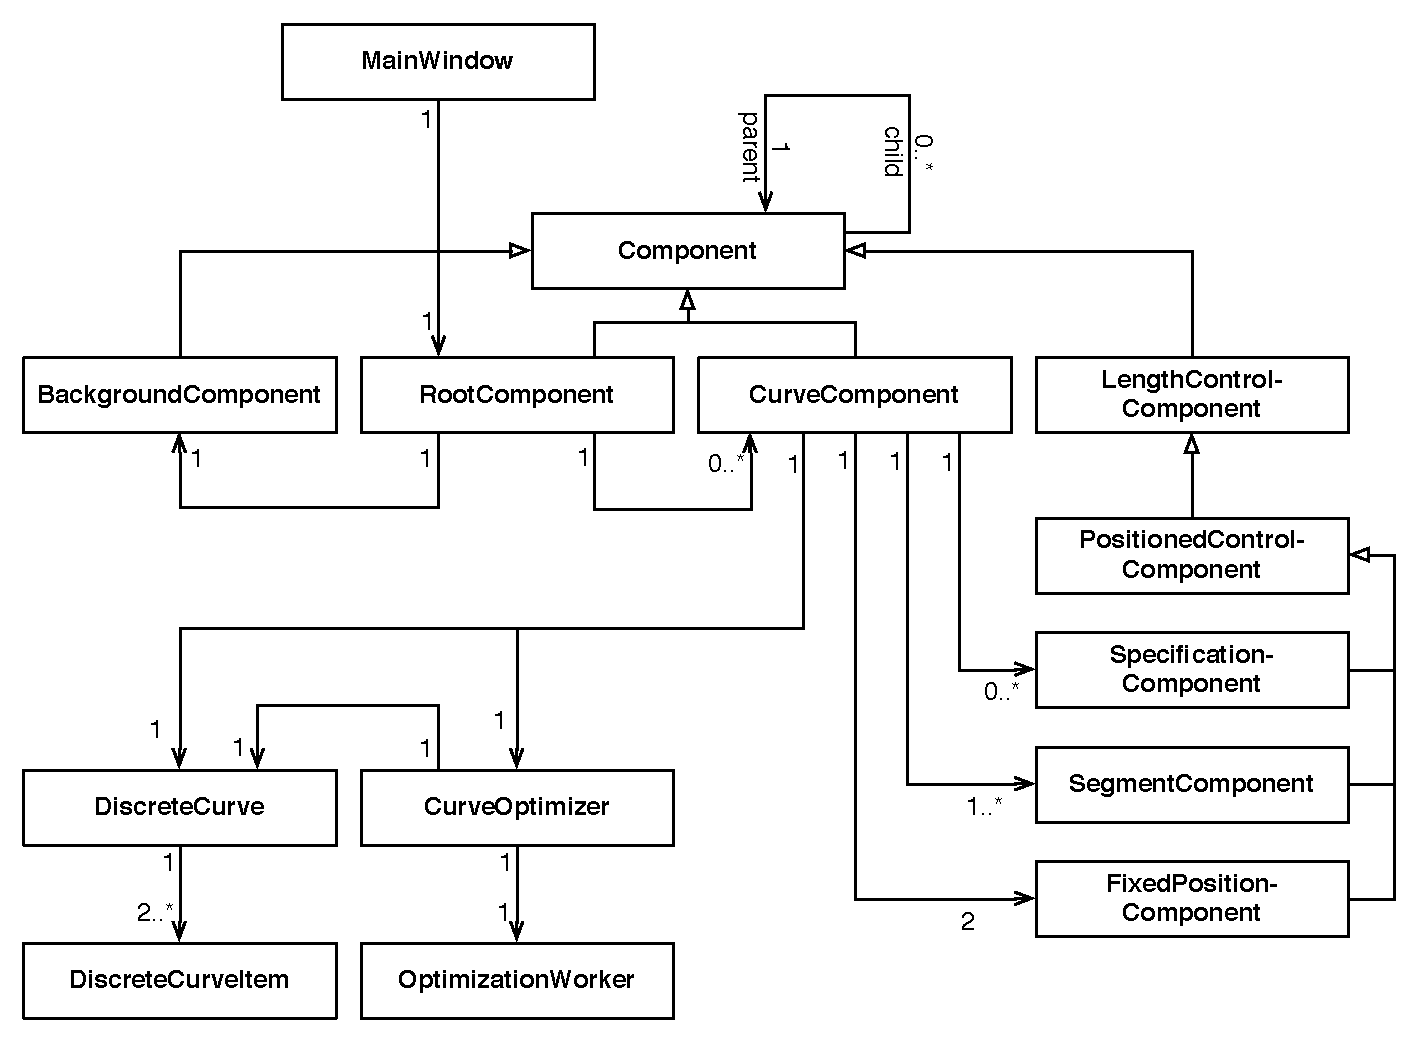
\includegraphics[width=\textwidth]{../resources/ui_components_class_diagram.pdf}
					\caption{Class Diagram of the User Interface Components}
					\label{figure:ui_components_class_diagram}
				\end{figure}
				
				Kurve's user interface constructed from Components. Components may contain a number of subcomponents, render themselves into a GTK\# context, and handle mouse and keyboards events. 
				\begin{itemize} 
					\item MainWindow - The MainWindow is a GTK\# window that contains the RootComponent. It triggers redraws of the RootComponent when appropriate (e.g. when the window is resized) and forwards mouse and keyboard events to the RootComponent.
					\item Component - Component is the abstract base class of all components that make up Kurve's user interface. It provides default implementations for rendering components, handling mouse and keyboard events, and provides a mechanism to trigger redraws of subcomponents.
					\item RootComponent - The RootComponent manages a list of CurveComponents and implements functionality to add and remove curve components. Additionally, the RootComponent implements save and load functionality.
					\item BackgroundComponent - This component can display a background image. This can be used to trace existing images with the Kurve tools.
					\item CurveComponent - This component represents a curve in the user interface. It consists of any number of PositionedControlComponents (any number of SpecificationComponents and a FixedPositionComponent at both the start and the end of the curve). This yields segments of the curve - one segment between each pair of PositionedControlComponents. These segments are represented by SegmentComponents. A CurveComponent uses a CurveOptimizer to create a curve from the specifications given by the SpecificationComponents. It implements functionality to add and remove SpecificationComponents and to change the curve template used (e.g. change the degree of the polynomial template). 
					\item LengthControlComponent - A LengthControlComponent is a Component that can modify the length of the Curve in a certain area.
					\item PositionedControlComponent - A PositionedControlComponent is a component that has a specific position on the curve. 
					\item SpecificationComponent - A SpecificationComponent allows to specify constraints on a curve. A point, direction and/or curvature can be specified for a given position using various mouse and keyboard commands. SpecificationComponents are visualized as a small black box that can be selected.
					\item FixedPositionComponent - FixedPositionComponents represent the start and end of a CurveComponent.
					\item SegmentComponent - A SegmentComponent represents a section of a curve delimited by two PositionedControlComponents. The SegmentComponent renders the curve in that segment, but it also allows to modify the length of the curve in that segment.
					\item DiscreteCurve and DiscreteCurveItem - A DiscreteCurve represents the data necessary to render a curve in the user interface. It contains information about the curve's points, direction, and curvature. It is represented by a number of DiscreteCurveItems that sample a source curve's point, direction and curvature at certain positions. 
					The CurveOptimizer yields this type of curve. The reason why this kind of discrete curve is used is because the Curve objects and the Optimizer (from the Kurve.Curves subsystem) cannot be used at the same time. This, in turn, is caused by the CasADi library, which is not thread safe. However, CasADi is used for representing Curves internally, as well as for performing optimization tasks.
					As Kurve uses a background thread to optimize curves, it is not possible to use the Curve objects yieded by the optimizer to render the curves in the main thread at the same time. For that reason, Curve objects are converted to DiscreteCurve objects in that background process.
					\item CurveOptimizer and OptimizationWorker - As the optimization process required to generate a curve from specifications takes too much time to perform in the main thread (the user interface would be blocked for too long), optimization is performed in a background thread. Each CurveComponent uses a CurveOptimizer to submit changed specifications. A single shared OptimizationWorker handles the synchronization and makes sure each submitted specification gets processed one by one. It is necessary to ensure that no optimization processes run in parallel, as the CasADi library (which is used in this process) is not thread safe.
				\end{itemize}

			\subsection{Usage}
				
				The user interface does not focus on user friendliness. Its purpose is to test the validity of the approach to curve design researched in this project. For that reason, most actions are performed using keyboard shortcuts. Many user interface elments can be selected with the mouse; this enables to use keyboard shortcuts that affect that component only. It is possible to interact with some components using the mouse. However, there is no toolbar or similar user interface elements that would make any of the features more accessible.
				
				The user interface allows the user to:
				\begin{itemize}
					\item add curves
					\item add specification controls to curves (specifying point, direction and/or curvature at a certain position on the curve) 
					\item control the curve's length (using specification and segment controls)
					\item control the degree of the polynomial template and the number of internal segments of the curve
					\item display a background image (e.g. to trace curves in an existing image)
					\item save and load curves
				\end{itemize}
				
				\begin{figure}[htb]
					\centering
					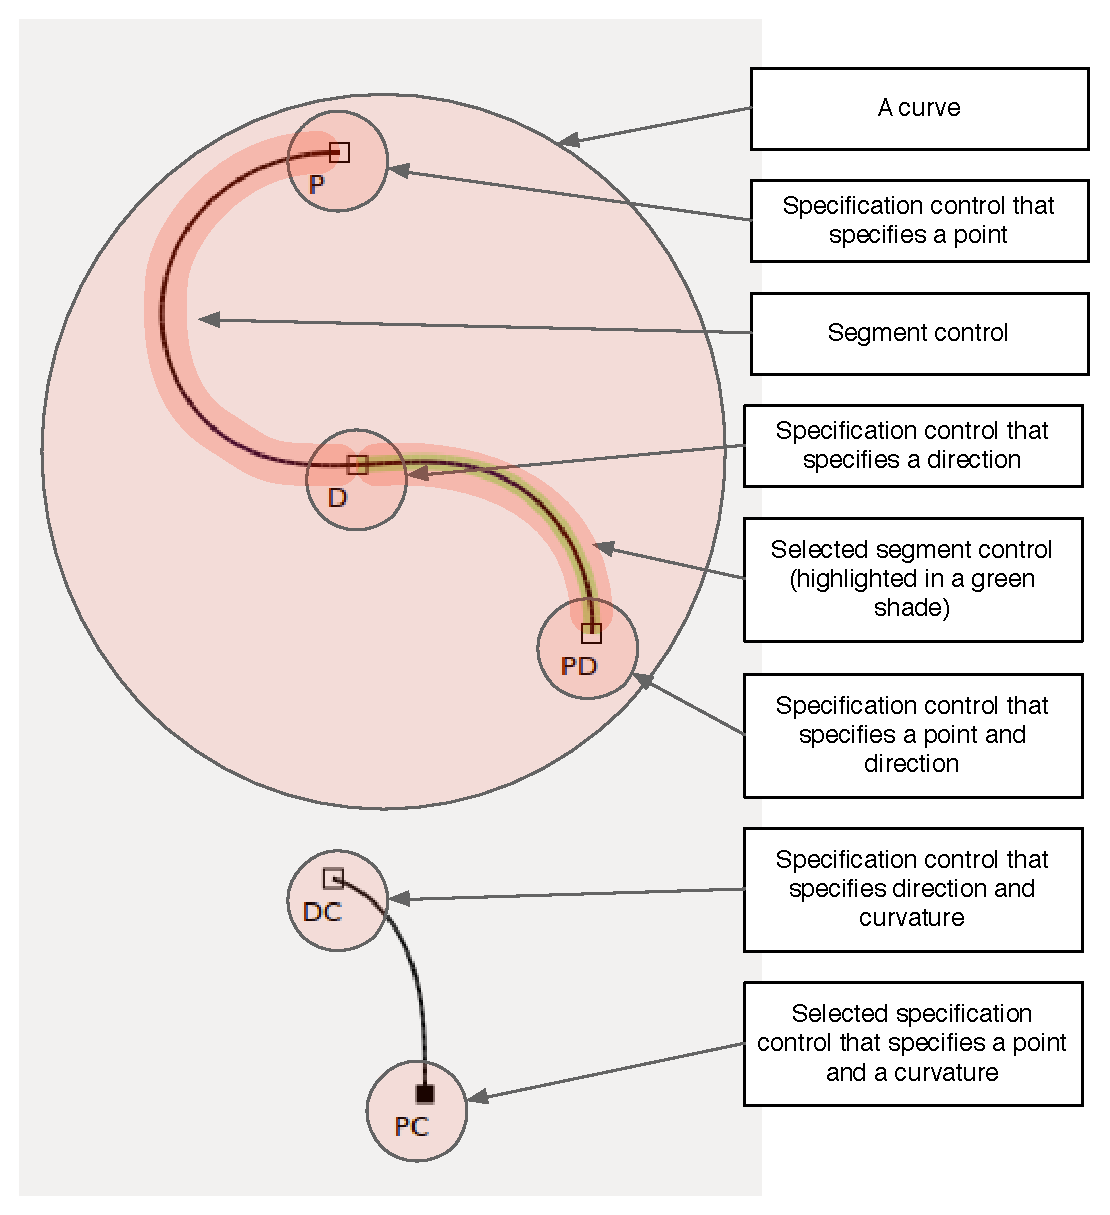
\includegraphics[width=\textwidth]{../resources/ui_components.pdf}
					\caption{Overview of the User Interface in Kurve}
					\label{figure:ui_components}
				\end{figure}
				
				\subsubsection{General Commands}
				
					A curve can be added by pressing `N'. A new Curve will appear in window that is initialized with a length of 100, and two specification controls specifying points. The curve uses one segment that uses a polynomial curve template with a degree of 10.
					
					To save all curves in the window, press `S'. A save file dialog will appear that allows the user to specify a filename. Saved files can later be loaded by pressing `L' which displays an open file dialog. Keep in mind that loading a file dismisses all curves in the current window.
					
					A background image can be displayed by passing a path to an image file when launching the Kurve application.
					
				\subsubsection{Curves}
					
					Click the right mouse button anywhere on a curve to add a specification control at that position. The newly added specification control does not yet specify anything. To remove a specification control, select it and press `R'. See the section \ref{section:specification_control} on how to use specification controls. 
					
					The length of the curve can be modified by selecting specification controls and segment controls and using the mouse wheel while pressing shift. If a specification control is selected, length is inserted to the left and right of the specification control; if a segment control is selected, that segment's length is changed.
					
					The current version of Kurve uses polynomials functions in each segment. The template that generates the functions and the number of segments can be modified as follows:
					
					\begin{itemize}
						\item To change the number of segments used, press `1' to decrease and `2' to increase the number of segments by one. ()
						\item To change the degree of the polynomial used in each segment, press alt + `1' to decrease, and alt + `2' to increase the degree by one.
					\end{itemize}
					Keep in mind that the segment count and the degree of the polynomial are not directly visible to the user and are used in the optimization process only. Adding more segments or increasing the degree of the polynomial allows more complicated curves, but has negative effects on the performance.
				\subsubsection{Specification Control}
				\label{section:specification_control}
				
					A specification control on a curve can specify any combination of a point, direction, or curvature at a certain position on the curve. Any combination of the three following letters represent which geometric attributes are specified by the specification control. 
					
					\begin{itemize}
						\item `P' indicates that a point that the curve has to pass through at that position is specified.
						\item `D' indicates that the direction of the curve at that position is specified.
						\item `C' indicates that the curvature of the curve at that position is specified.
					\end{itemize}
					
					Which attributes are specified can be toggled by selecting a specification component by clicking it and pressing the corresponding key on the keyboard. Which attributes are currently being specified is displayed in a label below the specification control. For example, if the label shows `n/a', nothing is specified, while `PC' indicates that a point and a curvature are specified.
					
					When a geometric attribute is specified by a specification control, it can be modified:
					
					\begin{itemize}
						\item Point: The point can be modified by dragging the specification control with the mouse.
						\item Direction: The direction can be modified using the mouse wheel.
						\item Curvature: The curvature can be modified by pressing the windows key while using the mouse wheel.
					\end{itemize}
					
					The position of the control can be modified by pressing the control key while using the mouse wheel. Keep in mind that when changing the position of a specification control that does not specify a point, the control itself will most likely move (and change its point).
					
					To achieve more fine-grained control, it is possible to press the alt key while performing any of the actions described above. This changes the affected property of the specification control more slowly. For example, if you press alt while dragging a specification control, it will move very slowly.
					
					As an experimental feature, it is also possible to change the position of a specification control by dragging it with the mouse while pressing shift. The position is calculated by the current state of the curve.
				
				\subsubsection{Segment Control}
				
					A segment control is a part of a curve delimited by either two specification controls or the start/end of the curve. It can be selected by clicking it.
					
					If at least one of the delimiting controls specifies a point, segments can be moved by dragging them with the mouse.
					
					A segment also displays the speed of the curve if it differs from the optimal speed. Too high speed is indicated by a red hue; this can usually be fixed by inserting additional length. Too low speed is indicated by a blue hue; usually there will be both blue and red sections. This usually indicates that the curve is too complex (i.e. there are too many specifications) to achieve a good representation with the current curve template. This can be fixed by either removing specifications, adding internal segments to the curve, or increasing the degree of the polynomial function template used in the curve.
				
				\begin{figure}[htb]
					\centering
					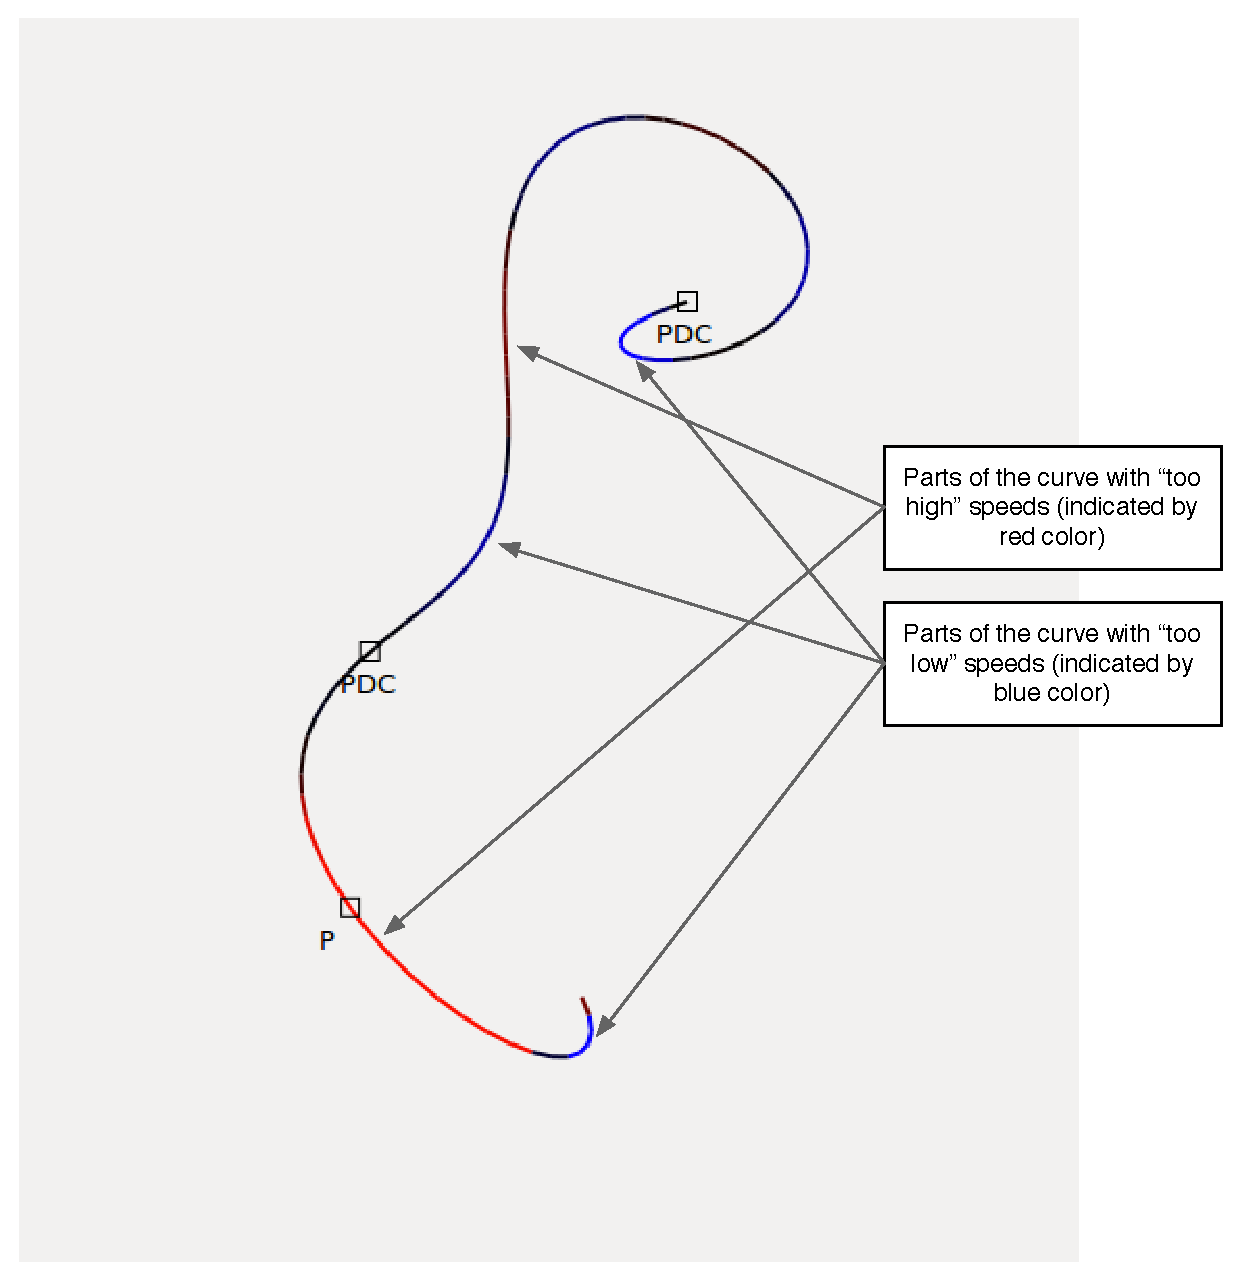
\includegraphics[width=\textwidth]{../resources/ui_speeds.pdf}
					\caption{Example of a Curve that is `Overspecified' (i.e. the speed of the curve cannot be kept constant due to the high amount of constraints)}
					\label{figure:ui_speeds}
				\end{figure}
				
				\subsubsection{Command Cheat Sheet}
					\begin{itemize}
						\item General
						\begin{description}
							\item[`N'] Add a new curve
							\item[`L'/`S'] Load/Save
							\item[`1'/`2'] decrease/increase internal segment count
							\item[Alt + `1'/`2'] decrease/increase polynomial template degree
						\end{description}
						\item All Controls
						\begin{description}
							\item[Click] Selects a control 
							\item[Shift + Click] Select multiple controls
							\item[Shift + Scroll (+ Alt)] Insert length at component (slowly)
						\end{description}
						\item Specification Control
						\begin{description}
							\item[Ctrl + Scroll (+ Alt)] Change the position of the specification (slowly)
							\item[Shift + Drag] Change position of specification (adjusts the point of the specification)
							\item[`R'] Removes the specification
							\item[`P'] Triggers point specification
							\item[Drag (+ Alt)] Move point (slowly). Only possible when point specification is enabled.
							\item[`D'] Triggers direction specification
							\item[Scroll (+ Alt)] Changes the direction (slowly). Only possible when direction specification is enabled.
							\item[`C'] Triggers curvature specification
							\item[Win + Scroll (+ Alt)] Changes the curvature (slowly). Only possible when curvature specification is enabled.
							\item[Shift + Click] Select multiple controls
							\item[Shift + Scroll (+ Alt)] Insert length at component (slowly)
						\end{description}
						\item Segment Control
						\begin{description}
							\item[Right-Click] Add empty specifcation control at that position
							\item[Drag] Moves any point specifications delimiting the segment. (Only possible if at leats one of the specification controls has the point specification enabled.)
						\end{description}
					\end{itemize}
		
	\section{Evaluation}
	\label{section:evaluation}

		The goal of this project was to explore possible improvements concerning the usability of curve design tools. The following sections discuss the results in this area.

		\subsection{Usability Analysis}
		\label{section:usability_analysis}

			Having applied the usability criteria from section \ref{section:usability_criteria_curve_design_tools} to Bézier splines and Spiro splines, we will now use them to evaluate usability aspects of our approach.

			\subsubsection{Expressiveness of the Specification Language}
			\label{section:expressiveness_specification_language}

				One of the primary goals of this project was to explore more expressive specification languages than those which are currently used in vector graphics software. To that end, our specification language supports specifying points, directions and curvatures at any number of positions on the curve, as well as the total length of the curve. This grants the user much flexibility in describing the source curve, allowing them to specify those properties that can describe the curve in the most concise fashion.

				The ability to specify curvature constitues a significant improvement over common curve design tools, where this is usually not possible. Using this functionality, the user can specify curves which are best expressed in terms of curvature in a natural and concise way. Not only does this make the curve design process less tedious, but it may also lead to better curves, since only the essential information about the curve is given to the software. This allows the fairness measure to choose the best possible curve, something that is not possible if lots of auxiliary information is supplied to the software in order to indirectly influence the curvature.

				Section \ref{section:specification_language} describes why it makes sense to specify the curve's total arc length. While fixing the arc length of the curve (and thus also the arc length between each specification item) may seem a little restrictive at first, there are actually quite a few upsides. For instance, by adjusting the arc length of a curve with a point specifications on each end, one can conveniently produce arcs between two points, since increasing the arc length will make the curve bulge out, with the fairness making sure that a smooth arc is produced.
				% Using common vector graphics software, one usually has to either risk an asymmetric and/or bumpy arc by specifying it using Bézier splines, or deal with some cumbersome tool for constructing elliptical arcs.
				Generally speaking, having control over the arc length of the curve results in benign and predictable curve behavior and is often useful for pulling it in place, not unlike the way one would handle a mechanical spline.

				On the other hand though, it is not possible not to specify the curve's arc length, and there may be cases where the user wants to leave it to the fairness measure to choose the best arc length for the curve. While it is sometimes possible to work around this issue by placing direction and/or curvature specifications instead of point specifications, that may not always be the case and further investigation into how arc length specification can be made optional while avoiding the problems mentioned in section \ref{section:specification_language} seems advisable.

				As a final way of demonstrating the high expressiveness, it may be noted that it is actually possible to specify segments of the Euler spiral using the specification language. As described in section \ref{section:fairness_measure}, the MVC fairness measure prefers constant or linearly changing curvature. Since every curve with linearly changing curvature is some segment of the Euler spiral, it is easy to specify those using the specification language by leaving the curve otherwise unconstrained.

			\subsubsection{Human Interaction with the Specification Language}
			\label{section:human_interaction_specification_language}

				The specification language is based on the familiar differential geometric properties point, direction, curvature and arc length, all of which have a simple geometric interpretation and are thus easy to understand.

				Points, directions and curvatures are easy to extract from some source curve. While extracting the arc length of a long curve may be somewhat difficult, this is usually not required since the arc length is mostly adjusted locally, where it is fairly easy to estimate.

				Since curves can usually be described using only a few specificaitons, communicating this information to the curve design tool is not too difficult either. Points are well-suited to be specified using the mouse pointer. The current prototype curve design tool only supports very basic input facilities for direction and curvature, making it somewhat difficult to create and modify these specifications. This is easily fixed though by utilizing their geometric interpretation, letting the user specify tangent lines and osculating circles instead of raw numeric values. Arc lengths are usually specified locally and by repeatedly making small adjustments, making them relatively easy to handle.

			\subsubsection{Smoothness and Minimality of Curves Selected by the Fairness Measure}
			\label{section:smoothness_minimality_curves_selected_fairness_measure}

				As described in section \ref{section:fairness_measure}, the MVC fairness measure the intuitive notion of smoothness very well, resulting in aesthetically pleasing curves.

				Unfortunately, the nonlinear optimization approach to finding the best curve can only find local optima, such that in many cases, the curve is not minimal, often containing loops and unnecessary inflection points. However, this is usually easy to fix by adjusting the specifications in such a way that the global optimum is found. For instance, a loop in the curve can often be removed by placing an additional point specification on the loop, pulling it away from the curve until the curve is forced to straighten out and finally removing the point specification again. Once the curve has been pushed into the global optimum like this, it is usually very stable.

			\subsubsection{Ability to Derive Curves from Descriptions}
			\label{section:ability_derive_curves_descriptions}

				As mentioned in section \ref{section:curve_derivation}, using nonlinear optimization has many advantages for research and proof of concept projects like this one. Unfortunately, the flexibility it grants comes with a price, in that it is much slower and also less reliable than unique mathematical constructions like the ones used for Bézier splines.

				Even on very powerful computers, running nonlinear optimization on splines with many segments and/or polynomials of high degree is too slow for interactive curve design, with updates taking more than 5 seconds. Most curves are very simple and do not need this kind of complexity, but for those that do, the bad performance can be very disruptive.

				Another issue is reliability. For some descriptions, the iterative optimization algorithm may converge extremely slowly or not at all, thus not producing a curve. In some cases, it is possible that small changes in the description restore the ability to converge on a solution, but sometimes one simply has to start over. There are also cases where the optimization gets stuck in a pathological local optimum, in which case one usually has to start over aswell.

				All these issues cause the prototype curve design tool to be somewhat impractical for actual curve design work, making this the primary issue with the chosen approach.

		\subsection{Examples}
		\label{section:examples}

			% fluttershy's mane
			%   spirals done this way are guaranteed to be smooth and not have any unintentional bumps
			%   comparison with bézier
			%     source image is in flash, already made of bézier splines, easy to trace
			%     still many more nodes needed
			%     hard to get actual, perfect spirals right
			%     curvature incontinuities, small bumps
			%     a bézier node comes with 2 handles, making it 3 points, or 6 scalar values that are specified, compared to 2 scalars for a DC specification
			%   somewhat hampered by poor performance and optimization stability issues, concept seems very powerful though
			% lugia profile view / lugia's back line (curled up)
			%   profits from global fairness optimization and curvature continuity guarantees
			%   some curves are more easily described in terms of curvature than points and/or direction
			% example of stability issues

		\subsection{Verdict}
		\label{section:verdict}

			% idea seems good, optimization issues get in the way
			% maybe move this to conclusion

	\section{Conclusion}
	\label{section:conclusion}

		% most issues stem from the optimization approach
		%  may make it hard to actually rate usability of the idea behind this
		% distinguish between further research work and turning the project into practical software)	
		% further possibilities to instantiate overall structure (different and/or combined spline primitives, constructive instead of optimization approach)
		% adaptive line segments, adaptive bézier approximation
		% steps that are necessary to turn this project into a useful application
		%   make absolutely sure the concept works by testing it with actual users
		%   performance improvements
		%   inkscape plugin
		% possibility to have curves without fixed length? could be useful for curves which only have specifications at the start and/or end of the curve
		% investigate into the calculus of variations and whether there may be a possibility to construct MVC curves based on our specification format, once the format itsself has proven to be useful
		% performance

		%   possible improvements
		%     make sure substitutions only happen where and when necessary
		%     cache partially instantiated IpoptProblem? such that fewer substitutions have to happen when changing a single specification
		%     use better linear solver with ipopt
		%     properly configure ipopt options
		%     adaptive segment density
		%     adaptive velocity/fairness trapezoid sum

	\clearpage

	\appendix

	\section{Definitions}
	\label{section:definitions}

		This section contains definitions used in the rest of the document.

		\subsection{Plane Vectors}
		\label{section:plane_vectors}

			A few basic definitions about vectors in the euclidean plane are needed:
			\begin{align*}
				\overline{\cdot} & : \function{\R{2}}{\R{2}} & \overline{v}      & = \vectorB{-v_2}{v_1}      && \text{orthogonal vector}\\
				\alpha           & : \function{\R{2}}{\RR}   & \apply{\alpha}{v} & = \apply{\atan2}{v_2, v_1} && \text{polar coordinate angle}
			\end{align*}

		\subsection{Parametric Curves}
		\label{section:parametric_curves}

			Parametric curves are described using functions \(\phi : \function{\unit}{\R{n}}\), called the parametrization function. The represented curve is then the image of this function. While there are many ways to parametrize a given curve, that is, represent it using a parametrization function, we are usually interested in those which yield a sufficiently smooth parametrization function, allowing for the concise description of curve properties using differential geometry.

		\subsection{Parametric Plane Curves}
		\label{section:parametric_plane_curves}

			In the special case of parametric plane curves, that is, parametric curves in the euclidean plane, we can define the following functions:
			\begin{align*}
				\phi    & : \function{\unit}{\R{2}} &                    &                                                && \text{point}\\
				\sigma  & : \function{\unit}{\RR}   & \apply{\sigma}{t}  & = \xn{\apply{\phi'}{t}}                        && \text{speed}\\
				\lambda & : \function{\unit}{\RR}   & \apply{\lambda}{t} & = \integral{0}{t}{\apply{\sigma}{u}}{u}        && \text{covered arc length}\\
				\delta  & : \function{\unit}{\RR}   & \apply{\delta}{t}  & = \apply{\alpha}{\apply{\phi'}{t}}             && \text{direction}\\
				\chi    & : \function{\unit}{\RR}   & \apply{\chi}{t}    & = \frac{\apply{\delta'}{t}}{\apply{\sigma}{t}} && \text{curvature}
			\end{align*}

			Using these definitions, the direction \(\apply{\delta}{t}\) is equal to the tangent angle at the point \(\apply{\phi}{t}\). If the curve is locally a straight line at the point \(\apply{\phi}{t}\), the curvature \(\apply{\chi}{t}\) is equal to \(0\). Otherwise, the curvature \(\apply{\chi}{t}\) is equal (up to sign) to the inverse of the radius of the osculating circle at the point \(\apply{\phi}{t}\).

		\subsection{Continuity}
		\label{section:continuity}

			The first way to define continuity of parametric curves is by simply transferring the notion of continuity from calculus as applied to the parametrization function. This leads to the notion of parametric continuity, denoted by \(\contp{n}\), stating that the \(n\)th derivative of the parametrization function is continuous.

			One may notice that this notion of continuity is a little too strict. A curve may look arbitrarily smooth, while its parametrization does not even have \(\contp{1}\) continuity, since the derivatives of the parametrization function may have discontinuities that do not manifest themselves in the curve that they represent. If that is the case, one can always find a different parametrization of the same curve that does not have these discontinuities. This insight gives rise to the definition of geometric continuity, denoted by \(\contg{n}\), which only requires that there exists a reparametrization of the parametric curve which is \(\contp{n}\) continuous.

			It follows immediately that every parametric curve that is \(\contp{n}\) continuous is also \(\contg{n}\) continuous. One may also observe that \(\contp{0}\) continuity and \(\contg{0}\) continuity are equivalent, since discontinuities in the parametrization function itsself manifest themselves directly in the curve it represents, and thus have to exist in all parametrizations of this curve. In the case of parametric plane curves, using the definitions from section \ref{section:parametric_plane_curves}, we can equate \(\contg{0}\) continuity with \(\phi\) being continuous, \(\contg{1}\) continuity with \(\delta\) being continuous and \(\contg{2}\) continuity with \(\chi\) being continuous.

	\clearpage

	\begin{thebibliography}{}

		\bibitem{thesis-mvc}
			\emph{Minimum Curvature Variation Curves, Networks, and Surfaces for Fair Free-Form Shape Design}\\
			Hentry Packard Moreton\\
			University of California, Berkeley, 1992

		\bibitem{thesis-spiro}
			\emph{From Spiral to Spline: Optimal Techniques in Interactive Curve Design}\\
			Raphael Linus Levien\\
			University of California, Berkeley, Fall 2009

		\bibitem{paper-mec}
			\emph{The Curve of Least Energy}\\
			B. K. P. Horn\\
			Massachusetts Institute of Technology, January 1981

		\bibitem{fluttershy}
			\emph{Fluttershy}\\
			Hasbro, Inc.\\
			My Little Pony: Friendship is Magic, 2010

		\bibitem{lugia}
			\emph{Lugia}\\
			Nintendo Co., Ltd.\\
			Pokémon, 1999

	\end{thebibliography}

\end{document}
